\documentclass[11pt]{article}

\usepackage[margin=1in]{geometry}
\usepackage{amsmath,amssymb,amsthm}
\usepackage{booktabs}
\usepackage{array}
\usepackage{microtype}
\usepackage{xurl}
\usepackage{pgfplots}
\pgfplotsset{compat=1.18}
\setlength{\emergencystretch}{1em}
\usepackage{enumitem}
\usepackage{natbib}
\usepackage[hidelinks]{hyperref}

\newtheorem{proposition}{Proposition}
\newcommand{\R}{\mathbb{R}}
\newcommand{\dd}{\mathrm{d}}
\newcommand{\KDM}{\ensuremath{\mathrm{KDM}}}
\newcommand{\LEDH}{\ensuremath{\mathrm{LEDH}}}
\newcommand{\GenUT}{\ensuremath{\mathrm{GenUT}}}
\newcommand{\OT}{\ensuremath{\mathrm{OT}}}

\title{Younis Kernel Mixtures and Model-Score Estimation\\
From the LEDH--OT--GenUT Filter to Corrected Mixtures}
\author{BayesFilter research note}
\date{11 September 2026}

\begin{document}
\maketitle

\begin{abstract}
A differentiable particle filter can compute the derivative of its own
finite likelihood accurately while estimating the underlying model score
poorly. This distinction explains both the progress and the negative results
of the BayesFilter investigation of Younis and Sudderth's kernel mixtures.
The original observation sidecar led to a complete kernelized-observation
recursion and then to an all-components, raw-importance-weight resampling
reference. The integrated derivatives pass their declared checks, but the
calibrated resampling construction has higher model-score mean squared error
than the canonical filter in both tested matrix-Gaussian scopes. We retain
these results and derive a different use of the same mixture ideas: construct
evaluable proposals, retain the original transition and observation densities
in the importance correction, and estimate the observed-data score by
averaging complete-data scores over possible ancestors. Selective pathwise
and importance-weight derivatives, valid control variates, and analytic
conditional integration supply additional variance-reduction candidates.
The note documents the implemented finite programs, the reasons for each
change in direction, the complete proposed recursions, and the experiments
needed to distinguish improved model-score accuracy from implementation
correctness. The new combination is a research proposal; its finite-particle
bias and computational value remain to be measured.
\end{abstract}
\clearpage
\tableofcontents
\clearpage

\section{The model score and the finite filter}
\label{sec:question}

The scientific question is how to estimate the score of a state-space model
accurately enough to support inference about its parameters. The existing
BayesFilter calculation uses \LEDH{} particle flow, PF--PF importance weights,
entropy-regularized \OT{}, Contract--E moment restoration, and \GenUT{}
higher-moment correction with two trust-region caps. These mechanisms define
a particular finite calculation. They are useful starting points for a
proposal, but they do not define what the exact model score must be.

This note grew out of the historical ``Section 3.6'' observation-sidecar
document. That earlier note remains in the isolated
\path{section-3-6-prior-weight-sidecar} worktree, under
\path{docs/papers/section_3_6_prior_weight_sidecar/}. The present manuscript,
\path{docs/papers/ledh_younis_kdm_score/ledh_younis_kdm_score.tex}, is its
broader successor. It brings together the subsequent implementation, results,
and the September 11 change in research question. The implementation history
is tied to research commit \texttt{804616e3}; later differences in the current
checkout, \texttt{5cc59cfa}, are identified in Section~\ref{sec:implementation}.

For fixed observations $y_{1:T}$ and model parameters $\theta\in\R^p$, write
\begin{align}
 \ell(\theta)&=\log p_\theta(y_{1:T}), &
 s(\theta)&=\nabla_\theta\ell(\theta), \label{eq:exact-score}\\
 L_0^N(\theta;\xi)&=\text{value of the executed finite filter}, &
 S_0^N(\theta;\xi)&=\nabla_\theta L_0^N(\theta;\xi).
 \label{eq:finite-score}
\end{align}
Here $N$ is the particle count and $\xi$ is the fixed random design used by
the finite program. In this note $\dd F$ means the directional derivative
$v^\mathsf{T}\nabla_\theta F$ for a declared direction $v$; $s$ denotes the
complete vector. Checking $S_0^N$ against finite differences of $L_0^N$ tests
the implementation of that derivative. Comparing it with $s$ tests its
accuracy as a model-score estimator. A third calculation, developed in
Section~\ref{sec:fisher}, estimates $s$ through posterior expectations. It
need not equal $S_0^N$ for the same particle realization.

For a fixed dataset, define the conditional bias and covariance of the
finite-program score by
\begin{equation}
 b_N(\theta;y)=\mathbb E_\xi[S_0^N\mid y]-s(\theta),\qquad
 V_N(\theta;y)=\operatorname{Cov}_\xi(S_0^N\mid y).
 \label{eq:conditional-score-error}
\end{equation}
When the second moments exist, its squared Euclidean error has expectation
$\|b_N\|^2+\operatorname{tr}V_N$. An individual discrepancy from Kalman does
not identify which term is responsible. Averaging errors over different
observation paths answers another question again: conditional biases can
cancel across datasets. Repeated filter randomizations within each dataset
are needed to distinguish conditional bias from Monte Carlo variance.

Even an unbiased likelihood estimate does not generally give an unbiased
log-likelihood score. Consider the positive estimator
$\widehat Z(\theta)=\theta+\varepsilon$, where
$\Pr(\varepsilon=a)=\Pr(\varepsilon=-a)=1/2$ and $\theta>a>0$.
Its mean is $Z(\theta)=\theta$, and its derivative is exactly one. Yet
\begin{equation}
 \mathbb E\left[\partial_\theta\log\widehat Z\right]
 =\frac12\left(\frac1{\theta+a}+\frac1{\theta-a}\right)
 =\frac{\theta}{\theta^2-a^2}\ne\frac1\theta
 =\partial_\theta\log Z.
 \label{eq:unbiased-value-biased-score}
\end{equation}
At $\theta=2$ and $a=1/2$, the two scores are $8/15$ and $1/2$.
The bias is created by the random denominator, despite correct
differentiation and an unbiased numerator. This example does not say that
every finite-particle score is biased in every model. It shows why the two
correctness statements cannot be substituted for a score-accuracy argument.

There are consequently several possible repairs. Missing derivatives of the
state, covariance, initial law, or sampling distribution require an
implementation or estimator correction. A reset or kernel that changes the
filtering measure requires a correction to that approximation or an explicit
new target. A valid but noisy integral requires better integration. The
development below separates these explanations before selecting the next
method. A zero-mean control variate addresses the last problem; it does not
remove an arbitrary bias already present in its baseline.

The existing implementation names remain useful for identifying what ran.
\texttt{ATOM-FINITE} denotes $L_0^N$; \texttt{KDM-FINITE} denotes a
positive-bandwidth observation program; \texttt{RESKDM-IWSG-FINITE} denotes
the post-Contract--E resampling program with raw anchored ratios; and
\texttt{RESKDM-SN-FINITE} denotes its historical, prematurely normalized
variant. \texttt{MODEL-IS} denotes an importance calculation whose numerator
retains the original model factors. These are program identities, not levels
of scientific validity. In particular, a correct \texttt{MODEL-IS} update
does not by itself make an additional deterministic reset unbiased, and a
different finite derivative is acceptable only under its actual name.

The \LEDH{} spelling follows the Li--Coates particle-flow construction
\citep{li2017particle}; the differentiable-transport context is
\citet{corenflos2021differentiable}. The new investigation now includes
alternative model-score estimators explicitly. It no longer rules them out
merely because they differentiate a different finite scalar.


\section{The executed atom program}
\label{sec:atom}

Let $x_{t,i}^{-}$ and $w_{t,i}^{-}$ denote the cloud and normalized weights
immediately before the observation update.  The finite program can be written
schematically as
\begin{align}
 x_{t,i}^{-}
   &= \Phi_{t,\theta}(x_{t-1,i}^{+},\xi_t), \\
 x_{t,i}^{\mathrm{out}}
   &= F_{t,\theta}^{\mathrm{LEDH}}(x_{t,i}^{-};\xi_t), \\
 a_{t,i}
   &= \log w_{t,i}^{-}
      +\log p_\theta(x_{t,i}^{\mathrm{out}}\mid x_{t-1,i}^{+})
      +\log g_\theta(y_t\mid x_{t,i}^{\mathrm{out}})
      +\log |J_{t,i}|
      -\log q_{t,\theta}(x_{t,i}^{-}\mid x_{t-1,i}^{+},y_t), \\
 Z_t
   &= \sum_{i=1}^{N}\exp(a_{t,i}), \\
 w_{t,i}^{+}
   &= \exp(a_{t,i})/Z_t, \\
 x_t^{+}
   &= R_\theta(x_t^{\mathrm{out}},w_t^{+};\xi_t), \label{eq:atom-program}\\
 L_0^N(\theta;\xi)
   &= \sum_{t=1}^{T}\log Z_t,\qquad
 S_0^N(\theta;\xi)=\nabla_\theta L_0^N(\theta;\xi).
\end{align}
Here $x_{t,i}^{\mathrm{out}}$ is the post-flow state, $J_{t,i}$ is the
forward flow Jacobian, and $q_{t,\theta}$ is the pre-flow proposal density.
$\Phi$ includes the declared transition and UKF covariance lifecycle, while
$F^{\mathrm{LEDH}}$ is the flow map; the displayed terms make the PF--PF
correction explicit.  In a
bootstrap/no-flow special case, the proposal and transition terms cancel and
$a_{t,i}=\log w_{t,i}^{-}+\log g_\theta(y_t\mid x_{t,i}^{-})$.  The reset $R$
includes the Sinkhorn/\OT{} map, Contract--E moments, \GenUT{} corrections,
and the dual-cap trust-region map.  This form matches the canonical score
route, whose weight logits contain transition, observation, log-determinant,
and proposal terms.  No such term may be silently dropped from the value or
its tangent.

For the auxiliary sidecar it is useful to expose the same code path as a
prior-observation factorization.  Define
\begin{align}
 b_{t,i} &= \log w_{t,i}^{-}
      +\log p_\theta(x_{t,i}^{\mathrm{out}}\mid x_{t-1,i}^{+})
      +\log |J_{t,i}|
      -\log q_{t,\theta}(x_{t,i}^{-}\mid x_{t-1,i}^{+},y_t),\\
 B_t &= \log\sum_i\exp(b_{t,i}),\qquad
 \bar w_{t,i}=\exp(b_{t,i}-B_t),\\
 a_{t,i} &= b_{t,i}+\log g_\theta(y_t\mid x_{t,i}^{\mathrm{out}}),\qquad
 Z_t=\sum_i\exp(a_{t,i}).
 \label{eq:prior-observation-factorization}
\end{align}
The implementation records $\bar w_t$ as
\texttt{prior\_observation\_weights}; these are the weights that may be
used with a new observation functional.  The posterior weights in
\eqref{eq:atom-program} are $w_t^+$ and must not be reused as $\bar w_t$.

The derivative in \eqref{eq:finite-score} is a total derivative.  Thus a
tangent through $x_t^{-}$, $w_t^{-}$, the observation factor, the \OT{} map,
the Contract--E residual design, the higher moments, and the dual caps is
included whenever that dependence is part of the declared finite scalar.
Holding a cloud fixed and differentiating only the observation factor is a
different partial derivative.

The executable analytical endpoint evaluates one arbitrary parameter
direction per call.  For a scalar parameter this number is the score.  For
$p>1$, a full score vector requires $p$ calls with the model tangent set to
the coordinate directions (or another spanning basis); each call is still a
total derivative through the entire finite recurrence.  The Phase~4A and Phase~4B score-quality fixtures have one parameter.
The later adapter audit exercises coordinate and mixed directions for five
models through the two-step endpoints. Those checks cover the derivative
components, but do not establish a scalable batch implementation of the full
score vector.

The research snapshot exposes the following analytical function and
its legacy row-mapped batch wrapper:
\begin{itemize}[leftmargin=2em]
  \item \texttt{canonical\_value\_and\_analytical\_score}\\
        \path{bayesfilter/highdim/ledh_canonical_score_tf.py};
  \item the batch wrapper
        \texttt{canonical\_batch\_value\_score}\\
        \path{bayesfilter/highdim/ledh_canonical_batch_}\\
        \path{tf.py}.\\
        It accepts both the historical \texttt{substeps} keyword and the
        authority-aligned \texttt{flow\_substeps} alias, and rejects
        conflicting values.
\end{itemize}
The separate lower-level GenUT candidate/diagnostic is:
\begin{itemize}[leftmargin=2em]
  \item \texttt{finite\_value\_score}\\
        \path{bayesfilter/highdim/cubature_genut_filter.py}.
\end{itemize}
Calling it is not evidence that the LEDH PF--PF flow and Contract--E reset
were executed.  The registry mismatch found during the audit has been repaired:
the registry now names the exported
\texttt{canonical\_value\_and\_analytical\_score}, and the governance test
resolves every registered entry point to a callable.  This closes discovery
only; it does not implement KDM or prove numerical score validity.  The existing
Section~3.6 prior-weight sidecar is diagnostic work from an isolated worktree;
it is not an integrated route in this checkout and is not a Younis IWSG
implementation through the reset.  The analytical function defaults to
\texttt{reset\_policy=none}, a diagnostic slice.  A canonical baseline
invocation must explicitly select \texttt{reset\_policy=contract\_e} and the
owner-registered dual-cap and trust-region settings.

\section{What the Younis construction supplies}
\label{sec:younis}

The mixture resampling and fixed-proposal importance gradient below follow
\citet[Section~4, equations (14)--(15)]{younis2023}. We distinguish that
construction from its later integration with BayesFilter resets and scores.


Younis and Sudderth begin with a weighted empirical cloud and replace its
Dirac representation by a regularized mixture
\begin{equation}
 \mu_h^N(\dd z)
   = \sum_{i=1}^{N} w_i k_{B_i}(z-x_i)\,\dd z,
 \qquad
 m_\theta(z)=\sum_{i=1}^{N}
       w_i(\theta)k_{B_i(\theta)}(z-x_i(\theta)).
 \label{eq:kdm}
\end{equation}
For their mixture-density particle filter, this mixture replaces discrete
resampling.  With a common Gaussian bandwidth one may generate an anchor
sample by
\begin{equation}
 I_j\sim\operatorname{Cat}(w_1,\ldots,w_N),\qquad
 z_j=x_{I_j}+L\varepsilon_j,\qquad
 \varepsilon_j\sim N(0,I),\quad LL^\mathsf{T}=B.
 \label{eq:younis-sampling}
\end{equation}
The 2024 construction stratifies the uniforms used for the categorical draw.
The label $I_j$ generates the sample, but the differentiable density is the
marginal sum in \eqref{eq:kdm}; it is not the density of the selected
component.  Thus every component can contribute to the gradient at every
sample location.  This is the source of the $N$-by-$N$ work in a
gradient-bearing resampling step.

Their IWSG construction fixes a proposal at the current parameter value.  With
\begin{equation}
 q_0(z)=m_{\theta_0}(z),\qquad
 \rho_j(\theta)=\frac{m_\theta(z_j)}{q_0(z_j)},\qquad
 z_j\sim q_0,
 \label{eq:iwsg-ratio}
\end{equation}
the finite estimator of a mixture expectation and its derivative are
\begin{align}
 \widehat I(\theta)
   &=\frac{1}{M}\sum_{j=1}^{M}\rho_j(\theta)\phi_\theta(z_j),\\
 \dd\widehat I
   &=\frac{1}{M}\sum_{j=1}^{M}
       \left\{\dd\rho_j\,\phi_\theta(z_j)
              +\rho_j\,\dd\phi_\theta(z_j)\right\}.
 \label{eq:iwsg}
\end{align}
At $\theta=\theta_0$, $\rho_j=1$.  The locations $z_j$ are held fixed in
this differentiation; parameter dependence is represented by the mixture
density ratio.  This is not the total JVP of an inverse-CDF draw or of a
parameter-dependent component index.  Equations~\eqref{eq:iwsg-ratio}--
\eqref{eq:iwsg} establish the derivative of a mixture expectation.  They do
not by themselves establish the derivative of an arbitrary nonlinear
operation that couples the complete set $(z_1,\ldots,z_M)$.  For such an
operation $H_\theta$, ordinary importance sampling on the joint sample would
instead use
\begin{equation}
 R_M(\theta)=\prod_{j=1}^M\rho_j(\theta),\qquad
 \dd\{R_M H_\theta\}\big|_{\theta_0}
 =\dd H_{\theta_0}+H_{\theta_0}
   \sum_{j=1}^M\dd\log m_\theta(z_j)\big|_{\theta_0}.
 \label{eq:joint-mixture-ratio}
\end{equation}
This joint ratio is exact for an expectation under independent mixture draws,
but its variance can grow rapidly with $M$.  Feeding individual IWSG weights
through a nonlinear \OT{} reset defines a finite weighted-particle algorithm;
it is not silently promoted to the joint identity
\eqref{eq:joint-mixture-ratio}.

The ratio in \eqref{eq:iwsg-ratio} is a raw importance weight.  Replacing it
by the self-normalized ratio
\begin{equation}
 \bar\rho_j(\theta)=\frac{\rho_j(\theta)}{\sum_l\rho_l(\theta)}
 \label{eq:self-normalized-ratio}
\end{equation}
changes the finite estimator.  At the anchor,
$\dd\log\rho_j=\dd\log m_\theta(z_j)$, whereas
\begin{equation}
 \dd\log\bar\rho_j
 =\dd\log m_\theta(z_j)
  -\frac1M\sum_l\dd\log m_\theta(z_l).
 \label{eq:centered-ratio-tangent}
\end{equation}
The second expression has been centered by a random sample average and is not
Equation~(15) of Younis and Sudderth.  Their released MDPF code confirms the
same ordering: it constructs the unnormalized gradient-injection factor
$\exp\{\log m-\operatorname{stop}(\log m)\}$, multiplies that factor by the
next measurement and dynamics weights, and only then normalizes the posterior
weights \citep{youniscode2023}.  The source code's small additive numerical
constant is an engineering detail and is not part of the mathematical route
defined here.

For a Gaussian component, let $u_i=z-x_i$.  Its complete directional
differential is
\begin{equation}
 \dd\log k_{B_i}(u_i)
 =
 u_i^\mathsf{T}B_i^{-1}\dd x_i
 +\frac12\left[
   u_i^\mathsf{T}B_i^{-1}(\dd B_i)B_i^{-1}u_i
   -\operatorname{tr}(B_i^{-1}\dd B_i)
 \right].
 \label{eq:component-tangent}
\end{equation}
Therefore
\begin{equation}
 \dd m_\theta(z)
 =\sum_i\left[
       (\dd w_i)k_{B_i}(u_i)
       +w_i k_{B_i}(u_i)\dd\log k_{B_i}(u_i)
     \right]. \label{eq:mixture-tangent}
\end{equation}
Equation~\eqref{eq:mixture-tangent} is the term that a KDM score path must
carry for every cloud, weight, or bandwidth dependence declared to vary with
$\theta$.  A bandwidth or cloud may instead be a genuinely fixed numerical
design, in which case its zero tangent is part of the scalar's definition.
Stopping a dependence that the declared scalar retains is a partial
derivative; declaring a quantity fixed before defining the scalar is not.

The source papers establish this mixture-gradient construction for learned,
discriminative state-density objectives.  In particular, the 2023 MDPF uses
the mixture both for posterior-state loss evaluation and for resampling; the
2024 paper again gives the marginalized ratio and separates resampling and
posterior bandwidths.  Neither paper derives the observed-data score of a
generative state-space model, an \LEDH{} flow, an \OT{} reset, \GenUT{}
moments, or dual-cap constraints.  Their complexity discussion makes the
computational boundary explicit: evaluating the mixture gradient at every
resampled location creates all-pairs interactions.  The papers' linear-cost
inference path sets forward resampling weights to uniform and does not compute
these gradients.  It cannot be transplanted to a score path without a new
approximation and error analysis.

\section{Why positive bandwidth is a target change}

The atom cloud is
\begin{equation}
 \mu_0^N(\dd z)=\sum_i w_i\delta_{x_i}(\dd z).
 \label{eq:atom-measure}
\end{equation}
For a test function $\phi$,
\begin{equation}
 \int\phi(z)\mu_h^N(\dd z)
 =\sum_i w_i\int\phi(x_i+u)K_{B_i}(\dd u),
 \label{eq:smoothed-functional}
\end{equation}
which is not generally $\sum_i w_i\phi(x_i)$.  This gives the following
simple boundary.

\begin{proposition}
Suppose the kernel weights are nonnegative and sum to one, and each kernel
is centered with finite covariance $B_i$. If $w_i>0$ and $B_i\ne0$ for at
least one component, the atom and kernel measures differ. Their parameter
derivatives therefore require separate justification; a positive-bandwidth
calculation is not, by its construction, the derivative of the atom program.
\end{proposition}

\begin{proof}
Take $\phi(z)=\|z\|^2$. Centering eliminates the cross term in
$\|x_i+u\|^2$, so the difference between the two expectations is
$\sum_i w_i\operatorname{tr}(B_i)>0$. Unequal parameterized expectations
can nevertheless have equal derivatives at particular points, or even differ
by a constant. Thus this measure argument proves a change of functional, not
a universal pointwise inequality of scores. Equality of the scores would need
an additional argument for the actual parameterized functional.
\end{proof}

A limiting theorem as bandwidth tends to zero would concern convergence;
it would not make two finite-bandwidth programs exactly equal.

The case $B=0$ is an explicit atom branch, not a request to evaluate a
singular Gaussian density.  A zero-bandwidth parity test must therefore not
form a Cholesky factor or an inverse of $B=0$ and then infer that the result is
the atom program.

For a linear-Gaussian observation model, a Gaussian state kernel gives the
useful exact convolution
\begin{equation}
 \overline g_\theta(y\mid x,B)
 = \int g_\theta(y\mid x+u)N(u;0,B)\,\dd u
 = N\!\left(y;C_\theta x,\,
       R_\theta+C_\theta B C_\theta^\mathsf{T}\right).
 \label{eq:linear-convolution}
\end{equation}
Write
\begin{align}
 S_i &= R_\theta+C_\theta B_i C_\theta^\mathsf{T}, &
 \mu_i &= C_\theta x_i, &
 r_i &= S_i^{-1}(y-\mu_i).
\end{align}
For fixed data $y$, the total directional differential used below is
\begin{align}
 \dd\mu_i
   &= (\dd C)x_i+C\,\dd x_i,\\
 \dd S_i
   &= \dd R+(\dd C)B_iC^\mathsf{T}
      +C(\dd B_i)C^\mathsf{T}+CB_i(\dd C)^\mathsf{T},\\
 \dd\log \overline g_i
   &=r_i^\mathsf{T}\dd\mu_i
     +\frac12\left\{
       r_i^\mathsf{T}(\dd S_i)r_i
       -\operatorname{tr}(S_i^{-1}\dd S_i)
     \right\}.
 \label{eq:linear-convolution-tangent}
\end{align}
Thus state, observation-map, observation-covariance, and bandwidth tangents
are all required when those quantities vary.  Positive semidefinite $B_i$ is
permitted here, including rank-deficient $B_i$, because only the strictly
positive definite observation covariance $S_i$ is factored.  This statement
does not assert an ambient Lebesgue density for a singular state kernel.
The corresponding observation increment
\begin{equation}
 \overline Z_t
 =\sum_i w_{t,i}^{-}\overline g_\theta(y_t\mid x_{t,i}^{-},B_{t,i}),
 \qquad
 \overline L_h^N=\sum_t\log\overline Z_t
 \label{eq:smoothed-value}
\end{equation}
is a well-defined new finite program.  It equals the atom increment only at
zero bandwidth or in special accidental cases.  If it is fed into the
subsequent reset, it defines an even larger new program.

The same distinction applies to a KDM placed after the reset.  Replacing
$x_t^+$ by a draw from \eqref{eq:kdm} changes the input to the next
transition and therefore changes all later normalizers.  The change may be
scientifically useful, but it is not an implementation detail.

\section{From Section 3.6 to the integrated experiments}
\label{sec:history}

The earliest question was whether an inexpensive smooth observation
functional could provide useful score information alongside the GenUT
filter. The Section 3.6 sidecar was designed as a separate deterministic
proposal force, with the canonical value retained for endpoint correction.
That was a legitimate mechanics experiment, but it was not a construction of
the canonical total score and it never supplied a known-mean control variate.

Its first repair concerned observation timing. Let $w_i^-$ be normalized
weights before the current observation, $g_i$ its likelihood at particle $i$,
and $Z=\sum_i w_i^-g_i$. The posterior weights are $w_i^+=w_i^-g_i/Z$.
The historical capture hook ran before reset but after this observation
update. Reusing its $w_i^+$ in a second likelihood average therefore gave
\begin{equation}
 \widetilde Z=\sum_iw_i^+g_i
 =\frac{\sum_iw_i^-g_i^2}{Z},\qquad
 \widetilde Z-Z=\frac{\operatorname{Var}_{w^-}(g)}{Z}.
 \label{eq:historical-double-observation}
\end{equation}
For two equally weighted particles with likelihoods 1 and 3, the intended
increment is 2, while the reused posterior weights give 2.5. The word
``pre-reset'' did not make the captured weights pre-observation. The repaired
sidecar used the actual prior observation weights and differentiated its
declared observation covariance dependence, while holding the captured cloud,
weights, and kernel fixed. It remained a conditional derivative.

The September 3 pilot used one-step diagonal LGSSMs: $(d,N,T)=(1,4,1)$ and
$(3,6,1)$. Four calibration paths and eight streams per scope selected the
grid boundary $\rho=0.8$; eight disjoint validation paths and eight streams
per scope supplied the holdout comparison. The recorded relative
path-level squared-bias changes were 6.6082 with interval
$[-0.2825,19.4854]$ and 0.2209 with interval $[-0.9342,1.5096]$.
Both intervals crossed zero, and the recorded stream-MCSE ratios, ranging
from 0.1756 to 0.4709, failed the threshold 0.10. These tiny CPU/non-XLA
diagnostics supplied no ranking or bias-reduction evidence. Separate
reversibility and volume checks passed at about machine precision, but
proposal mechanics did not establish score accuracy, HMC mixing, or posterior
correctness. The sidecar remained isolated and unpromoted.

The next stages sought to remove the conditional-derivative restriction.
Phases 1--3 implemented complete mixture differentials, a fixed-chart support
reference, and an auxiliary functional constructed from the actual canonical
trace. Phase 4A then fed kernelized observation weights and their tangents
through the complete reset. Phase 4B added the source paper's mixture
resampling mechanism after Contract--E and carried the resulting weights and
covariance marks into later time steps. These changes made the full feedback
testable. They also defined new finite programs; no residual correction made
them equal to the original atom program.

The chronology therefore does not support a claim that a control variate was
completed and then simplified. The executed work moved from an auxiliary
conditional functional to separately named integrated experiments. This was
useful for determining whether those mechanisms improved model-score error.
It did not solve the original target-preserving control-variate problem.
The negative results below are the reason to reconsider the insertion point
and the score estimator together.


\subsection{Phase 4A: integrated kernelized observation weighting}

The first integrated experiment replaces only the point observation factor in
\eqref{eq:prior-observation-factorization}.  With the ordinary
pre-observation PF--PF logit $b_{t,i}$, define
\begin{align}
 a^h_{t,i}&=b_{t,i}+\log\overline g_\theta(
   y_t\mid x_{t,i}^{\mathrm{out}},B_{t,i}),\\
 Z^h_t&=\sum_i\exp(a^h_{t,i}), &
 \alpha^h_{t,i}&=\exp(a^h_{t,i})/Z^h_t,\\
 L_{\mathrm{obsKDM}}^N&=\sum_t\log Z^h_t, &
 S_{\mathrm{obsKDM}}^N&=\dd L_{\mathrm{obsKDM}}^N.
 \label{eq:observation-kdm-program}
\end{align}
Its one-step tangent is
\begin{align}
 \dd\log Z^h_t
 =\sum_i\alpha^h_{t,i}
   \left(\dd b_{t,i}+\dd\log\overline g_{t,i}\right),\qquad
 \dd\alpha^h_{t,i}
 =\alpha^h_{t,i}\left[
   \dd a^h_{t,i}-\dd\log Z^h_t\right].
 \label{eq:observation-kdm-weight-tangent}
\end{align}
The executed program passes $(x_t^{\mathrm{out}},\dd x_t^{\mathrm{out}},
\alpha_t^h,\dd\alpha_t^h)$ into the existing Contract--E reset and the
existing \GenUT{}/dual-cap correction.  Their output and tangent feed the next
time step.  Equations~\eqref{eq:linear-convolution-tangent} and
\eqref{eq:observation-kdm-weight-tangent} therefore define a total derivative
of this complete finite program, not a conditional observation derivative.

The reset also carries the particle-local UKF covariance with the same
target-by-source transport used for the state.  If $A_{ri}$ is the normalized
Sinkhorn transport from source particle $i$ to reset particle $r$, then the
covariance recursion and its total tangent are
\begin{align}
 P'_{r} &= \sum_i A_{ri}P_i, &
 \dd P'_{r} &= \sum_i (\dd A_{ri})P_i+
                    \sum_i A_{ri}\dd P_i.\label{eq:covariance-carry}
\end{align}
The carried $P'_r$, not the old source ordering, is consumed by the next UKF
prediction.  Here $P_i$ denotes a particle-local conditional covariance; no
between-cloud scatter term is added.  This same-transport carry is the
declared Contract--E extension of categorical triple resampling.  A previous
implementation omitted it at the analytical endpoint; that call-chain bug
was repaired and is now covered by endpoint and two-step tests.

This program is deliberately called \emph{kernelized observation weighting}.
It is not the complete Bayesian update of a Gaussian mixture: it does not
propagate the conditional posterior mean and covariance of every mixture
component.  It is consequently not a full Younis mixture-density particle
filter.  Positive bandwidth is labelled \texttt{KDM-FINITE}; the explicit
$B=0,\dd B=0$ branch is labelled \texttt{ATOM-FINITE} and must reproduce the
canonical trajectory.

A second insertion point represents the post-reset cloud by a continuous
mixture before the next transition.  It defines the distinct
\texttt{RESKDM-IWSG-FINITE} scalar and is derived and implemented separately
in the next subsection; it is not part of the Phase~4A
observation-weighting scalar.

The first paired experiment now answers the narrow Phase~4A question for one
small linear--Gaussian cell.  With $N=32$, $T=5$, 20 calibration paths, and
100 disjoint validation paths, calibration selected $\rho=0.8$ in
$B=\rho^2Q$.  The atom score MSE was $3.3366$ and the kernelized-observation
MSE was $3.4980$, a relative change of $-4.84\%$ when positive values denote
improvement.  The paired 95\% bootstrap interval for the MSE difference was
$[-0.223,0.597]$, so the two scores are not statistically ranked.  Inspection
of all prespecified bandwidths on this now-consumed holdout showed no positive
point improvement; $\rho=1.6$ was worse with interval $[0.189,2.399]$.

The mechanism is visible in the score errors.  From $\rho=0$ to $\rho=0.8$,
their sample standard deviation decreased from $1.616$ to $1.580$, but their
mean moved from $-0.868$ to $-1.014$.  The modest variance reduction was more
than offset by additional bias.  This rejects Phase~4A for promotion in this
scope.  It does not test the complete Younis resampling operation described
next, and it does not license tuning on the inspected validation paths.

For a finite IWSG normalizer,
\begin{align}
 \widehat Z_h(\theta)
   &=\frac{1}{M}\sum_j
       \rho_j(\theta)g_\theta(y_t\mid z_j),\\
 \dd\log\widehat Z_h
   &=\frac{\sum_j\rho_jg_j
       \left(\dd\log\rho_j+\dd\log g_j\right)}
           {\sum_j\rho_jg_j}.
 \label{eq:iwsg-normalizer}
\end{align}
Equation~\eqref{eq:iwsg-normalizer} is a derivative of the KDM
importance-sampling program.  It is not an identity with the atom program.

\subsection{Phase 4B: a complete mixture-resampling reference}

The source operation can now be stated without an ancestry ambiguity.  Let
$(c_{t,i},\alpha_{t,i},P_{t,i})$ denote the locations, normalized weights, and
particle-local UKF covariance marks presented to a continuous resampler.  If
the KDM replaces Contract--E, these are the weighted post-flow particles.  In
the combined BayesFilter reference selected below, they are the Contract--E
output, its carried covariances, and uniform weights
$\alpha_{t,i}=1/N$ with $\dd\alpha_{t,i}=0$.  In either case define the
marginalized resampling density
\begin{equation}
 m_{t,\theta}(z)=\sum_{i=1}^N
   \alpha_{t,i}(\theta)k_{B_t(\theta)}
      (z-c_{t,i}(\theta)).
 \label{eq:phase4b-mixture}
\end{equation}
The first reference uses the source paper's common Gaussian bandwidth and an
ordinary full-rank linear--Gaussian fixture.  The complete sequential route is
not called source-faithful because its Contract--E placement and covariance
marks are BayesFilter extensions.  A DSGE version must replace this density by
the chart density in Section~\ref{sec:support}.

At an anchor $\theta_0$, stratified categorical uniforms and Gaussian noises
generate fixed locations $z_{t,j}$ from $m_{t,\theta_0}$.  Component labels are
recorded to replay the draw, but are marginalized in every density evaluation.
For a nearby $\theta$, define
\begin{align}
 r_{t,j}(\theta)
   &=\frac{m_{t,\theta}(z_{t,j})}
           {m_{t,\theta_0}(z_{t,j})}, &
 \eta_{t,j}(\theta)
   &=\frac{1}{N}r_{t,j}(\theta),
 \label{eq:phase4b-iwsg-weights}\\
 \gamma_{t,ji}(\theta)
   &=\frac{\alpha_{t,i}k_{B_t}(z_{t,j}-c_{t,i})}
           {m_{t,\theta}(z_{t,j})}. &&
 \label{eq:phase4b-responsibilities}
\end{align}
At the anchor, $r_{t,j}=1$ and $\eta_{t,j}=1/N$.  The locations are fixed in the IWSG
differential, so $\dd z_{t,j}=0$, while
\begin{align}
 \dd\log r_{t,j}
   &=\sum_i\gamma_{t,ji}
      \left\{\dd\log\alpha_{t,i}
             +\dd\log k_{B_t}(z_{t,j}-c_{t,i})\right\},\\
 \dd\log\eta_{t,j}&=\dd\log r_{t,j}, &
 \dd\eta_{t,j}&=\eta_{t,j}\dd\log r_{t,j}.
 \label{eq:phase4b-weight-tangent}
\end{align}
Equations~\eqref{eq:component-tangent} and
\eqref{eq:phase4b-weight-tangent} include the cloud, weight, and bandwidth
terms.  Evaluating all $\gamma_{t,ji}$ is the required $N^2$ operation.  The
sum of the $\eta_{t,j}$ tangents is generally nonzero for a finite sample;
forcing it to zero would replace the raw IWSG correction by
\eqref{eq:self-normalized-ratio}.

Younis's particles carry locations and weights, not the UKF covariance used by
the LEDH implementation.  The following mark transport is therefore an
explicit BayesFilter extension:
\begin{align}
 \widetilde P_{t,j}
   &=\sum_i\gamma_{t,ji}P_{t,i}, &
 \dd\widetilde P_{t,j}
   &=\sum_i(\dd\gamma_{t,ji})P_{t,i}
     +\sum_i\gamma_{t,ji}\dd P_{t,i},\\
 \dd\gamma_{t,ji}
   &=\gamma_{t,ji}\left\{
       \dd\log\alpha_{t,i}+\dd\log k_{t,ji}
       -\dd\log m_{t,\theta}(z_{t,j})\right\}.
 \label{eq:phase4b-covariance-mark}
\end{align}
No between-component scatter is added: the kernel perturbation has already
been realized in $z_{t,j}$, and $P_{t,i}$ remains the local UKF algorithmic
mark.  This choice is testable, but it is not a result from the source paper.
The prespecified comparator instead carries the covariance mark of the fixed
anchor label,
\begin{equation}
 \widetilde P_{t,j}^{\mathrm{label}}=P_{t,I_{t,j}},\qquad
 \dd\widetilde P_{t,j}^{\mathrm{label}}=\dd P_{t,I_{t,j}}.
 \label{eq:phase4b-selected-mark}
\end{equation}
The label has no tangent.  Both policies retain the same marginalized mixture
density and raw IWSG weights; only the downstream UKF mark differs.  Neither
mark policy is supplied by Younis and Sudderth, so their comparison diagnoses a
BayesFilter extension rather than source fidelity.

That comparison is uninformative when all component marks and their tangents
are equal.  If $P_{t,i}=P_t$ and $\dd P_{t,i}=\dd P_t$, then
$\sum_i\gamma_{t,ji}=1$ and $\sum_i\dd\gamma_{t,ji}=0$ give
\begin{equation}
 \widetilde P_{t,j}=P_t,\qquad
 \dd\widetilde P_{t,j}
   =\Bigl(\sum_i\dd\gamma_{t,ji}\Bigr)P_t
      +\Bigl(\sum_i\gamma_{t,ji}\Bigr)\dd P_t
   =\dd P_t.
 \label{eq:phase4b-equal-marks}
\end{equation}
The fixed-label policy gives the same result.  Linear Gaussian prediction and
update preserve equal initial covariance marks, and normalized Contract--E
transport preserves their equality.  The matrix experiment below therefore
cannot select between these policies; floating-point differences in their
calibration scores have no scientific meaning.  Heterogeneous-mark tests are
needed to check the distinction, and nonlinear evidence is needed to choose
between them for a nonlinear filter.

There are now two possible placements, and they must not share a name.
Replacing Contract--E by mixture resampling gives the source MDPF placement
but removes the requested Contract--E, \GenUT{}, and dual-cap reset.  Retaining
Contract--E and then applying \eqref{eq:phase4b-iwsg-weights} before the next
transition executes both mechanisms.  The latter is the declared Phase~4B
BayesFilter reference.  Its fixed locations, raw IWSG weights, and covariance
marks become the parents of the next transition; all later PF--PF,
flow-Jacobian, reset, and cap terms are then differentiated normally.

To make the finite scalar explicit, let $h_{t+1,j}(\theta)$ contain the full
next-step PF--PF multiplier for child $j$: transition density, observation
density, flow Jacobian, and proposal denominator.  The post-resampling
increment is
\begin{equation}
 Z_{t+1}^{\mathrm{IWSG}}(\theta)
 =\sum_{j=1}^N\eta_{t,j}(\theta)h_{t+1,j}(\theta)
 =\frac1N\sum_{j=1}^N r_{t,j}(\theta)h_{t+1,j}(\theta).
 \label{eq:phase4b-next-normalizer}
\end{equation}
The posterior weights are normalized only after the product
$\eta_{t,j}h_{t+1,j}$ is formed.  This preserves the raw importance-sampling
normalizer in \eqref{eq:phase4b-next-normalizer}.  Call the resulting scalar
\begin{equation}
 L_{\mathrm{resKDM,IWSG}}^N(\theta;\xi,z^0,q^0)
 =\sum_{t=1}^T\log Z_t^{\mathrm{IWSG}},\qquad
 S_{\mathrm{resKDM,IWSG}}^N=\dd L_{\mathrm{resKDM,IWSG}}^N.
 \label{eq:phase4b-finite-target}
\end{equation}
This is the combined \texttt{RESKDM-IWSG-FINITE} program.  It is neither
$L_0^N$ nor the Younis MDPF alone.  A two-pass evaluation is required: an
anchor pass generates every sequential $z_{t,j}$ and denominator
$m_{t,\theta_0}(z_{t,j})$; a replay pass evaluates the same fixed sample bank
and its total tangent for other $\theta$.  Re-anchoring inside an HMC
trajectory would change the finite energy and is forbidden.

The raw IWSG weights are part of this new finite scalar, not auxiliary
metadata.  In particular, if $\omega_{t+1,j}$ denotes the incoming weight used
by the next PF--PF step, then
\begin{equation}
 \log\omega_{t+1,j}=\log r_{t,j}-\log N,\qquad
 \dd\log\omega_{t+1,j}=\dd\log r_{t,j}.
 \label{eq:phase4b-incoming-weight}
\end{equation}
The next normalizer must consume both quantities.  Resetting the numerical
weights to $1/N$ while retaining only the sampled locations, or retaining the
weight values while discarding their tangent, removes the IWSG mechanism.

Prematurely normalizing the ratios defines a different scalar.  Because the
subsequent posterior softmax removes common scale, the state and posterior
weight recurrences agree, but the accumulated normalizer does not.  With the
same samples and covariance-mark policy,
\begin{equation}
 L_{\mathrm{resKDM,SN}}^N
 =L_{\mathrm{resKDM,IWSG}}^N
  -\sum_{t=1}^{T-1}\log\left\{\frac1N\sum_{j=1}^N r_{t,j}\right\}.
 \label{eq:phase4b-self-normalized-difference}
\end{equation}
The first Phase~4B implementation computed this
\texttt{RESKDM-SN-FINITE} scalar.  Its finite-difference agreement was correct
for that scalar but did not validate the intended raw-IWSG score.  The repaired
route implements \eqref{eq:phase4b-incoming-weight}; an executable regression
requires a generally nonzero sum of raw weight tangents and rejects the
centered tangent in \eqref{eq:centered-ratio-tangent} as its incoming score.

There are also two distinct meanings of ``unbiased'' that must not be
conflated.  Equations~\eqref{eq:iwsg-ratio}--\eqref{eq:iwsg} give the ordinary
importance-sampling identity for a single mixture expectation.  For a
nonlinear function of the complete resampled cloud, the exact joint identity
is \eqref{eq:joint-mixture-ratio}.  The sequential use of raw individual
weights in \eqref{eq:phase4b-incoming-weight} follows the IWSG
gradient-injection ordering, while using their scale in a generative evidence
normalizer is a BayesFilter extension.  Its analytical derivative is the total
derivative of $L_{\mathrm{resKDM,IWSG}}^N$ as defined here, but neither the
source paper nor the present derivation proves that it is an unbiased estimator of
$\nabla_\theta\log p_\theta(y_{1:T})$, of the expected stochastic-filter loss,
or of $S_0^N$.  Those are empirical or additional-theory questions.

The zero-bandwidth limit requires separating the locations from their IWSG
derivative.  In this combined route, the component weights are exactly $1/N$
and the $j$th stratified position is $(j-1+u_j)/N$, with $0\le u_j<1$.
Consequently the selected label is $I_j=j$: each component is selected once.
The earlier statement that this particular route tends to repeated component
locations was wrong.  With $B=h^2Q$ and $L_QL_Q^\mathsf{T}=Q$, its anchor
sample is $z_j=c_j+hL_Q\varepsilon_j$, which tends to $c_j$.

This location limit does not establish score parity.  For distinct centres,
fixed positive-definite $Q$, and a parameter-independent bandwidth scale $h$,
the selected component dominates the mixture as $h\to0$.  At the anchor,
its leading location contribution to the IWSG differential is
\begin{equation}
 \dd\log m_\theta(z_j)\big|_{\theta_0}
 \simeq \frac{1}{h}\varepsilon_j^\mathsf{T}L_Q^{-1}\dd c_j.
 \label{eq:phase4b-small-bandwidth-tangent}
\end{equation}
Thus the fixed-sample tangent can grow while the forward locations converge.
Repeated centres require a separate mixture-limit analysis.  At $B=0$ the
ambient Gaussian density is undefined, so Phase~4B does not implement a
zero-bandwidth score branch equal to \texttt{ATOM-FINITE}.  Its checks are instead anchor
identity, complete-mixture density, analytical-versus-finite-difference
tangents, sequential replay, and comparison with both the canonical score and
the Kalman score.

The exact all-components reference costs $O(N^2)$ per mixture-gradient
evaluation and $O(TN^2)$ for a sequential gradient.  Sparse neighbors, random
features, and low-rank approximations would be new algorithms; they are not
permitted in the reference and require separate error analyses if considered
later.

\subsection{The matrix Gaussian score comparison}

The first score-quality campaign used a two-state model.  Its dynamics are
$x_t=A(\theta)x_{t-1}+\epsilon_t$, and its measurements satisfy
$y_t=Hx_t+\nu_t$.  The matrices are
\begin{align}
 A(\theta)
 &=
 \begin{bmatrix}0&0.12\\-0.08&0.10\end{bmatrix}
 +\theta\begin{bmatrix}1&0\\0&0.7\end{bmatrix},
 &\theta_0&=0.72,\\
 H&=\begin{bmatrix}1&0.25\\-0.15&0.9\end{bmatrix},
 &Q&=\begin{bmatrix}0.12&0.025\\0.025&0.09\end{bmatrix},\\
 R&=\begin{bmatrix}0.22&0.035\\0.035&0.18\end{bmatrix},
 &P_0&=\begin{bmatrix}0.8&0.12\\0.12&0.6\end{bmatrix}.
 \label{eq:phase4b-matrix-lgssm}
\end{align}
Here $x_{-1}\sim N(0,P_0)$ and the first observation follows one transition.
At $\theta_0$, $A(\theta_0)$ is stable.  An independent analytical Kalman
recursion differentiates its prediction, innovation covariance, gain, posterior
mean, and posterior covariance with $\dd A=\operatorname{diag}(1,0.7)$.  The
first particle scopes were $(N,T)=(32,5)$ and $(64,20)$.  The smaller scope ran
first; both scopes completed within the total compute budget.  This matrix
fixture replaces the earlier scalar proposal,
which was wrong for testing the full pairwise correction because that
correction is identically absent in one dimension.

Each scope used 40 calibration paths, 30 separate power-pilot paths, and 500
untouched validation paths.  The bandwidths selected from the declared grid
were $\rho=0.8$ and $0.4$, respectively.  Relative to the exact Kalman score,
the validation result was
\begin{center}
\begin{tabular}{lrrl}
\toprule
$(N,T)$ & Atom MSE & KDM MSE & KDM minus atom, 95\% interval\\
\midrule
$(32,5)$ & 3.94210 & 4.45250 & $[0.07106,\,0.94986]$\\
$(64,20)$ & 3.86260 & 10.13463 & $[5.10083,\,7.55881]$\\
\bottomrule
\end{tabular}
\end{center}
The intervals use 4,000 paired path bootstrap resamples.  They support higher
MSE for the calibrated KDM candidate in each tested scope.  Both frozen
low/high absolute-score groups also had higher KDM point MSE than the atom
and observation-KDM comparators; the high-score small-scope interval alone
crossed zero.  The simpler bootstrap particle comparator had larger MSE,
which does not rescue the loss to the unmodified filter.

The primary criterion required an interval demonstrating at least ten percent
MSE reduction.  Neither scope passed it.  The pilots requested 8,900 and
4,160 paths for the specified twenty-percent improvement alternative, so the
500-path cap also left both scopes underpowered for that design.  The
negative result is therefore a rejection of these calibrated candidates,
not a completed search over KDM methods.  Their numerical controls remain
unpromoted hypotheses, and changing $N$ and $T$ together does not isolate
either effect.  In the smaller scope, a slight observed variance reduction
was offset by greater squared bias; in the larger scope both increased.
These bias/variance decompositions are descriptive.  Small bandwidth was
especially unstable: the calibration MSE at $\rho=0.025$ reached
$1.63\times10^9$ and $9.18\times10^{35}$.  This is consistent with the
small-bandwidth tangent in \eqref{eq:phase4b-small-bandwidth-tangent}, not
evidence that a small value perturbation gives a small score perturbation.


The bootstrap entry differentiates the finite program along its realized,
fixed ancestor labels. It checks that program's derivative; it is not the
ancestor-averaged Fisher-score baseline developed in Section~\ref{sec:fisher}.
The canonical numerical controls were frozen campaign comparators and were
not independently optimized for each scope. The results therefore compare
the tested configurations. Since both $N$ and $T$ change between the two
scopes, the contrast does not isolate horizon dependence or particle-number
dependence. The reported subgroup intervals are pointwise, not simultaneous.

The raw-IWSG log-value shift relative to the atom program averaged
$-0.02449$ and $-0.02377$ in the two scopes, with mean squared shifts
$0.07284$ and $0.04023$. Small changes in a scalar do not imply small changes
in its derivative. These descriptive value differences therefore do not
rescue the failed score comparisons.

\subsection{Why the next direction changes}
\label{sec:pivot}

The tested all-IWSG candidate is rejected for the two matrix-Gaussian scopes.
Its derivative agrees with its declared finite program, yet its model-score
MSE is higher. In the smaller scope, the descriptive error mean and variance
changed from $-1.08143$ and $2.77816$ for the canonical score to $-1.32100$
and $2.71290$ for Phase 4B. In the larger scope they changed from $-0.98767$
and $2.89289$ to $-1.57710$ and $7.66270$. The second scope therefore shows
both more squared error in the mean and more variation across paths. These
across-path decompositions are descriptive; they do not separately estimate
the conditional bias at each fixed dataset.

The result is not adequately explained by saying that the KDM derivative is
different from the atom derivative. Both are candidates for approximating
the exact model score, and a different estimator could have smaller error.
The more useful question is why the new approximation should be closer to
the model. Adding Gaussian observation covariance changes the observation
factor. Adding a second reset changes future particles. Evaluating narrow
kernels with fixed-location importance gradients can amplify noise. None of
these operations, by itself, corrects the original model-score bias.

The earlier restriction to the executed finite derivative made unrelated
score recursions appear inadmissible. That restriction protected the meaning
of the canonical API, but it was too narrow as a research objective. A
Fisher-score estimator can be a valid candidate for the underlying model
without being the derivative of the existing OT-reset scalar. It must be
named and validated accordingly. Likewise, a centered control variate can
reduce variance without removing the bias of its baseline. The distinction
changes what an experiment must measure; it does not relax the mathematics.

One historical cost argument also needs correction. The Section 3.6 memo
grouped PaRIS with inherently quadratic ancestor calculations. The exact
ancestor sum is quadratic, but PaRIS replaces that sum with sampled backward
ancestors and has an expected linear-cost result under stated mixing and
acceptance assumptions \citep[Section 3.1, Algorithm 2; Section 3.2.4,
Theorem 10]{olsson2014paris}. Those assumptions do not hold automatically in
every repository model, particularly when transition densities are singular
or backward acceptance becomes small. Nevertheless, ``always quadratic''
was an incorrect reason to exclude it. The all-components IWSG experiments
already incurred quadratic work, making a measured comparison with
ancestor-averaged methods more relevant than that earlier exclusion suggests.

The next direction therefore assigns different jobs to three components.
An evaluable mixture proposes particles. The original model densities specify
their importance correction. A posterior-score recursion averages over the
ancestor uncertainty that remains. Selective pathwise and importance-weight
gradients are an additional way to reduce variance when mixture expectations
must be differentiated. This combination has not been tested here. It is
preferred as the next hypothesis because every component has a clear role in
the model-score calculation, not because the existing negative results prove
it will perform better.


\section{Mixture proposals with the original model correction}
\label{sec:model-mixtures}

There is a continuous mixture already present in a particle filter whenever
the physical transition has a continuous density. Let
$\{x_{t-1}^j,W_{t-1}^j\}_{j=1}^N$ approximate the filtering distribution
after observation $t-1$, with $\sum_jW_{t-1}^j=1$. Propagating that measure
through the actual transition density gives
\begin{equation}
 a_t(x)=\sum_{j=1}^N W_{t-1}^j f_\theta(x\mid x_{t-1}^j),\qquad
 u_t(x)=g_\theta(y_t\mid x)a_t(x).
 \label{eq:physical-predictive-mixture}
\end{equation}
The first density predicts the state; the second incorporates the current
observation but is not normalized. The transition's process covariance is
part of the model. It is not an artificial bandwidth added to make an atom
cloud differentiable. When $f_\theta$ is Gaussian, $a_t$ is already a Gaussian
mixture, so Younis-style mixture calculus can be studied on this physical
predictive distribution directly.

Choose an evaluable proposal $q_t$ whose support contains that of $u_t$, and
draw $x_t^i\sim q_t$. The correct importance calculation is
\begin{equation}
 v_t^i=\frac{u_t(x_t^i)}{q_t(x_t^i)},\qquad
 \widehat z_t=\frac1N\sum_i v_t^i,\qquad
 W_t^i=\frac{v_t^i}{\sum_k v_t^k}.
 \label{eq:model-marginal-weights}
\end{equation}
Conditionally on the incoming cloud and a proposal fixed before these draws,
\begin{equation}
 \mathbb E_{q_t}[\widehat z_t\mid\mathcal F_{t-1}]
 =\int \frac{u_t(x)}{q_t(x)}q_t(x)\,\dd x
 =\int u_t(x)\,\dd x.
 \label{eq:conditional-model-normalizer}
\end{equation}
Here $\mathcal F_{t-1}$ includes the previous weighted particles and any
proposal design fixed from them and the observed data. A kernel can change
where particles are drawn without changing the numerator in this identity.
The cancellation fails if the denominator is merely the density of the
selected component rather than the actual marginal proposal, or if the
proposal is refitted to the same draws without a justified adaptive weighting
scheme.

This is the useful connection to the marginal particle filter.
\citet[Algorithm 2, Theorem 2, equations (9)--(12)]{lai2022vmpf} integrate out
the ancestor index and evaluate full transition and proposal mixtures. Their
estimator-coupling argument establishes an unbiased likelihood normalizer for
the specified recursion. It also explains a local Rao--Blackwell variance
reduction; the paper explicitly does not claim that the complete MPF always
has lower variance than every corresponding SMC run. Its variational
objective, equation (13), is $\mathbb E\log\widehat Z$, which is not
$\log Z$. Unbiased differentiation of that objective would not settle the
model-score question in Section~\ref{sec:question}.

The associated author implementation evaluates the transition mixture with
\texttt{reduce\_logsumexp}, adds the observation log density, and subtracts
the proposal log density \citep{laicode2022}. These operations support
\eqref{eq:model-marginal-weights}. They do not establish compatibility with
BayesFilter's analytical derivative, initialization, GPU/XLA, or tuning
requirements. The proposed generative mixture route is not implemented by
merely calling the existing observation-KDM endpoint.

The distinction between numerator and proposal also determines how much of
the current LEDH machinery can be reused. Its flow, UKF information, GenUT
moments, and OT couplings may supply proposal centers, covariances, or
deterministic transformations. The numerator must still use the intended
incoming filtering weights and the actual transition and observation
densities. Replacing those weights by uniform reset weights and those states
by uncorrected reset locations changes $a_t$. Equation~\eqref{eq:conditional-model-normalizer}
then certifies an integral of that changed approximation, not the original
model recursion. A deterministic transformation may be used as a proposal
only when its induced density, including every necessary Jacobian, is known.

A defensive mixture can protect proposal support when a guided component
misses a plausible mode. For a fixed $0<\eta<1$, let
\begin{equation}
 q_t(x)=(1-\eta)q_t^{\rm guided}(x)+\eta a_t(x).
 \label{eq:defensive-mixture}
\end{equation}
Since $q_t\ge\eta a_t$, the incremental weight satisfies
$v_t(x)\le g_\theta(y_t\mid x)/\eta$. A bounded observation likelihood
therefore gives a bounded incremental weight. It does not bound every score
derivative, and the mixing fraction remains a scope-specific proposal choice
to calibrate. An arbitrary positive fraction is not justified as a default.

\subsection{An analytically adapted Gaussian example}

The first implementation can be checked in a model where the best local
proposal is available exactly. Suppose
$f_\theta(x\mid x_{t-1}^j)=\mathcal N(x;m_j,Q)$ and
$g_\theta(y_t\mid x)=\mathcal N(y_t;Hx,R)$, with $Q$ and $R$ positive
definite. In the matrix-LGSSM test, $m_j=A(\theta)x_{t-1}^j$.
Multiplying the two Gaussian densities gives
\begin{equation}
 f_\theta(x\mid x_{t-1}^j)g_\theta(y_t\mid x)
 =c_j\,\mathcal N(x;\widetilde m_j,\widetilde Q),
 \label{eq:adapted-component-product}
\end{equation}
where completing the square, or conditioning a joint Gaussian, yields
\begin{align}
 V&=HQH^\mathsf T+R,& c_j&=\mathcal N(y_t;Hm_j,V),\\
 K&=QH^\mathsf T V^{-1},&
 \widetilde m_j&=m_j+K(y_t-Hm_j),\\
 \widetilde Q&=Q-QH^\mathsf T V^{-1}HQ.&
 \label{eq:adapted-component-parameters}
\end{align}
The component evidence $c_j$ tells us how plausible ancestor $j$ is after the
new observation. Its conditional Gaussian moves the proposal toward that
observation. Thus the normalized predictive update is the mixture
\begin{equation}
 q_t^*(x)=\sum_j\frac{W_{t-1}^jc_j}{z_t^*}
                   \mathcal N(x;\widetilde m_j,\widetilde Q),
 \qquad z_t^*=\sum_j W_{t-1}^jc_j.
 \label{eq:fully-adapted-mixture}
\end{equation}
Substituting $q_t^*=u_t/z_t^*$ into
\eqref{eq:model-marginal-weights} makes every incremental weight equal to
$z_t^*$. The current-step proposal variance vanishes conditionally on the
incoming cloud. Earlier particle approximation remains, so this is not an
exact finite-particle Kalman filter. The example isolates the improvement
available from conditional integration and proposal adaptation before any
extra kernel smoothing is introduced. In particular, $Q$ here is the physical
process covariance, not the carried UKF mark or an added kernel bandwidth.

\subsection{Retained ancestry and a flow proposal}

The same model correction can be formulated on a joint ancestor--state
space. This is useful when the flow depends on the selected ancestor and
its inverse cannot be marginalized cheaply. The distinction determines the
correct numerator as well as the denominator; the following existing
\texttt{MODEL-IS} derivation is retained for that reason.


There is one direct KDM use that leaves the generative model factors in the
importance ratio, but it is a BayesFilter extension rather than the Younis
MDPF.  The treatment of ancestry must be fixed before writing the ratio.  If
an ancestor $A$ is retained, draw it with a frozen probability $r_{t,0}(a)$,
then draw a pre-flow state from a complete conditional mixture
$q^{\KDM}_{t,0}(x_0\mid a,y_t)$.  Apply the ancestor-specific LEDH map
$x_1=F_{t,\theta,a}(x_0)$, with forward Jacobian $J_{t,a}$.  The induced joint
proposal density is
\begin{equation}
 q_t(j,x_1)
 = r_{t,0}(j)q^{\KDM}_{t,0}(x_0\mid j,y_t)
   \,|\det J_{t,j}(x_0)|^{-1},
 \qquad x_0=F_{t,\theta,j}^{-1}(x_1).
 \label{eq:kdm-proposal-density}
\end{equation}
The corresponding unnormalised weight is
\begin{equation}
 \widetilde w_t
 = \frac{w^-_{t-1,J}
     f_\theta(x_1\mid x^+_{t-1,J})
     g_\theta(y_t\mid x_1)
     |\det J_{t,J}(x_0)|}
    {r_{t,0}(J)q^{\KDM}_{t,0}(x_0\mid J,y_t)}.
 \label{eq:kdm-proposal-weight}
\end{equation}
Here ``complete'' means the sum over every kernel component within the
conditional mixture for the retained ancestor, not the kernel of the component
that generated $x_0$.  If ancestry is marginalized instead, the numerator must
also be marginalized,
\begin{equation}
 \widetilde w_t(x_0)
 =\frac{g_\theta(y_t\mid x_1)|\det J_t(x_0)|
   \sum_a w^-_{t-1,a}f_\theta(x_1\mid x^+_{t-1,a})}
  {q^{\KDM}_{t,0}(x_0)}.
 \label{eq:kdm-proposal-marginal-weight}
\end{equation}
This second expression is valid only when the flow map does not depend on an
ancestor that has been marginalized.  Mixing a marginalized denominator with
the conditional numerator in \eqref{eq:kdm-proposal-weight} is wrong.

An auxiliary-particle lookahead may guide $r_{t,0}$, but its approximate
predictive likelihood cannot replace either the exact transition factor
$f_\theta$ or the observation factor $g_\theta$.  Under the usual support,
invertibility, and differentiation-under-the-integral conditions, the sample
average $\widehat Z_t$ and its derivative are unbiased for the one-step
particle predictive integral conditional on the incoming cloud.  The ratio
$\dd\widehat Z_t/\widehat Z_t$ is generally biased for its logarithmic
derivative.  Moreover, the deterministic Contract--E reset changes the next
incoming cloud, so this one-step identity is not a proof that the complete
finite-horizon algorithm is an unbiased likelihood or score estimator.

Following the fixed-denominator principle of Younis IWSG, this conditional
LEDH extension freezes $r_{t,0}$ and $q^{\KDM}_{t,0}$ at an anchor $\theta_0$ while
differentiating the model numerator and LEDH map.  Younis and Sudderth do not
derive this conditional LEDH construction.  If an implementation instead
recomputes the proposal as $\theta$ changes, it needs a separate derivation
that couples the sampling map, proposal density, ancestor selection, and state
map.  Merely subtracting proposal or selection log-density tangents from a
fixed-sample importance weight is wrong for the anchored model-normalizer
derivative.  This arm is therefore labelled
\texttt{MODEL-IS} and is compared separately with both the canonical
\texttt{ATOM-FINITE} score and the exact Kalman score.

At the atom reset itself, an ordinary density ratio cannot repair the change:
a finite atom measure and an absolutely continuous KDM are mutually singular.
A density-corrected KDM proposal can instead sample a continuous predictive
update, where the physical transition supplies the target density. Inserting
it directly at an atomic reset requires a different measure and an explicit
new target; the predictive-density argument does not correct that reset.

\section{A model score that averages over ancestors}
\label{sec:fisher}

A good proposal improves the particle approximation, but a separate question
remains: which score should we compute from those particles? Differentiating
every operation of a chosen finite filter is one answer. Fisher's identity
supplies another, aimed directly at the observed-data score.

Assume the initial, transition, and observation laws have differentiable
densities on a common dominating measure, and that differentiation may pass
through the joint integral. For $x_{0:T}$, the joint density is
\begin{equation}
 p_\theta(x_{0:T},y_{1:T})
 =\mu_\theta(x_0)\prod_{t=1}^T
       f_\theta(x_t\mid x_{t-1})g_\theta(y_t\mid x_t).
 \label{eq:joint-model-density}
\end{equation}
The derivative inside this density holds $x_{0:T}$ fixed. Define its complete
data score by
\begin{equation}
 H_T(x_{0:T})=\nabla_\theta\log\mu_\theta(x_0)
 +\sum_{t=1}^T\left\{
    \nabla_\theta\log f_\theta(x_t\mid x_{t-1})
   +\nabla_\theta\log g_\theta(y_t\mid x_t)\right\}.
 \label{eq:complete-data-score}
\end{equation}
Since $\nabla_\theta p_\theta=p_\theta H_T$, integrating this equality and
dividing by $Z=p_\theta(y_{1:T})$ gives
\begin{align}
 s(\theta)
 &=\frac{\int p_\theta(x_{0:T},y_{1:T})H_T(x_{0:T})\,\dd x_{0:T}}{Z}
 \notag\\
 &=\mathbb E_\theta[H_T(X_{0:T})\mid y_{1:T}].
 \label{eq:fisher-model-score}
\end{align}
The posterior expectation is over whole state histories, including the
initial state. A parameter-dependent stationary initial law contributes the
first term even when no observation is assigned to time zero. In a
latent-innovation representation, the density and the derivative must instead
be derived in those coordinates; the state-density expression cannot be used
unchanged for a singular transition.

The needed history average has a forward recursion. Let $H_t$ be
\eqref{eq:complete-data-score} truncated at time $t$, and define
$A_t(x_t)=\mathbb E[H_t(X_{0:t})\mid X_t=x_t,y_{1:t}]$. Conditional on
$X_t$, the observation at $t$ does not further distinguish its ancestors.
The backward conditional distribution is proportional to
$p_\theta(x_{t-1}\mid y_{1:t-1})f_\theta(x_t\mid x_{t-1})$.
Conditioning the additive score on this distribution gives
\begin{align}
 A_t(x)&=\nabla_\theta\log g_\theta(y_t\mid x)
 \notag\\[-2pt]
 &\quad+\int\left[A_{t-1}(z)
           +\nabla_\theta\log f_\theta(x\mid z)\right]
       p_\theta(z\mid x,y_{1:t-1})\,\dd z.
 \label{eq:fisher-conditional-recursion}
\end{align}
This is the step that a single realized ancestor cannot represent exactly.
It averages all histories compatible with the current state instead of
discarding them when a resampling label is selected.

For a weighted particle approximation, define the backward probabilities
\begin{equation}
 b_t^{ji}=
 \frac{W_{t-1}^j f_\theta(x_t^i\mid x_{t-1}^j)}
      {\sum_kW_{t-1}^k f_\theta(x_t^i\mid x_{t-1}^k)}.
 \label{eq:backward-particle-probabilities}
\end{equation}
All terms are evaluated at the current parameter; the denominator must be
positive. The initial particles must approximate $\mu_\theta$: they may be
drawn from it directly, or drawn from a covering proposal and weighted by
the corresponding initial-law ratio. Initialize
$A_0^j=\nabla_\theta\log\mu_\theta(x_0^j)$ and use
\begin{align}
 A_t^i&=\nabla_\theta\log g_\theta(y_t\mid x_t^i)
       +\sum_j b_t^{ji}\left[A_{t-1}^j
          +\nabla_\theta\log f_\theta(x_t^i\mid x_{t-1}^j)\right],\\
 \widehat s_N&=\sum_i W_T^i A_T^i.
 \label{eq:particle-fisher-recursion}
\end{align}
This is the marginal-score construction in
\citet[Section 2.2, Algorithm 2, equations (20) and (22)]{poyiadjis2011particle},
with the initial state indexed explicitly as time zero. Its relation to
modified differentiation rules is discussed by
\citet[Section 4.2, equations (24)--(25)]{scibior2021dpf}. The displayed
recursion follows directly from the conditional expectation above, with the
initial and observation timing made explicit.

No derivative of the proposal or of the sampled trajectory is missing from
\eqref{eq:particle-fisher-recursion}: its integrand is the complete-data
model score. Proposal design changes how well its expectation is estimated.
This differs from $S_0^N$, where state motion through the executed finite
program is part of the claimed derivative. The Fisher estimator should
therefore be checked against a model-score oracle and checked local density
derivatives. Requiring it to match finite differences of the old OT-reset
scalar would ask it to compute a different quantity.

Particle approximation and normalization still introduce error. With an
exact smoothing draw, $H_T$ is unbiased for $s$ under the stated integrability
conditions; with a finite approximate smoothing distribution,
$\widehat s_N$ is not generally unbiased. Averaging ancestors reduces a
particular source of randomness without proving a universal ranking of full
filters. This remains true when the marginal likelihood estimate itself is
unbiased.

The original Poyiadjis paper gives a useful, specific precedent. Its
Section~2.3 compares the methods against an analytic Gaussian-model score
using 500 particles and 100 replications. The discussion of linear growth in
the marginal method's variance combines a stability conjecture with those
numerical results; Theorem~1 instead proves a quadratic lower bound for the
genealogical construction under its stated mixing and boundedness conditions.
These distinctions prevent a local ancestor-averaging argument from becoming
an unsupported universal variance theorem for the proposed filter.

There is a useful computational overlap with
Section~\ref{sec:model-mixtures}. The transition mixture in the numerator
of \eqref{eq:model-marginal-weights} is also the denominator of
\eqref{eq:backward-particle-probabilities}. The same pairwise densities can
support both the value calculation and the score recursion. A direct
implementation costs $O(TN^2)$, plus the cost of the model derivatives.
Streaming reduces memory use, not the number of pairs. PaRIS is an option
for replacing the exact ancestor sum by a controlled number of backward
draws; its acceptance cost, added variance, and support assumptions must be
measured in the actual model before choosing it over the exact reference.

\subsection{Using both past and future information}

Younis and Sudderth's smoother suggests a complementary proposal design.
Their equation (18) draws from a mixture of forward and backward predictive
approximations, allowing either set of observations to nominate a state.
Their equation (19) retains a generative correction, including an auxiliary
reference density; equation (20) replaces its numerator with a learned
discriminative weight \citep[Section 4]{younis2024}. The distinction matters
here. A learned state predictor is not automatically a model posterior, and
multiplying two posterior approximations can count prior information twice
unless the appropriate reference-density factor is included.

For transition parameters, the score contains functions of
$(X_{t-1},X_t)$, so single-time smoothing marginals alone are insufficient.
A Younis-inspired smoother must supply adjacent-state or path information
and the original model correction. Its most direct role is therefore an
evaluable proposal for the expectation in \eqref{eq:fisher-model-score},
followed by model-based weighting, rather than replacement of that expectation
by the paper's supervised state-prediction loss. A learned proposal would
require its own target-specific training protocol and downstream validation.


\section{Selective mixture gradients and control variates}
\label{sec:hybrid}

The model-score recursion and the choice of mixture-gradient estimator are
separate decisions. Fisher's identity does not require differentiation of
every resampling draw. Mixture expectation derivatives may nevertheless be
needed for proposal learning, sensitivity calculations, or a separately
defined finite program. In those settings, using IWSG for every continuous
movement can introduce avoidable variance.

Consider a single component $Z=\mu+h\varepsilon$, with
$\varepsilon\sim\mathcal N(0,1)$ and fixed $h>0$. For the affine function
$\phi(z)=az+b$, the exact derivative of $\mathbb E\phi(Z)$ with respect to
$\mu$ is $a$. The location-score estimator and the pathwise estimator are
\begin{equation}
 G_{\rm IW}=(a\mu+b+ah\varepsilon)\frac{\varepsilon}{h},
 \qquad G_{\rm PW}=a.
 \label{eq:gaussian-gradient-estimators}
\end{equation}
Both have mean $a$. Using
$\mathbb E\varepsilon^2=1$, $\mathbb E\varepsilon^3=0$, and
$\mathbb E\varepsilon^4=3$ gives
\begin{equation}
 \operatorname{Var}(G_{\rm IW})
   =\frac{(a\mu+b)^2}{h^2}+2a^2,
 \qquad \operatorname{Var}(G_{\rm PW})=0.
 \label{eq:gaussian-gradient-variance}
\end{equation}
The constant part of the integrand, which has zero true derivative, is
responsible for the diverging term. Subtracting the detached baseline
$\phi(\mu)$ from the score-function term produces $a\varepsilon^2$, whose
variance is $2a^2$. No bias was removed; a needless source of variance was
removed. Figure~\ref{fig:gradient-variance} makes the bandwidth effect explicit.

\begin{figure}[tbp]
\centering
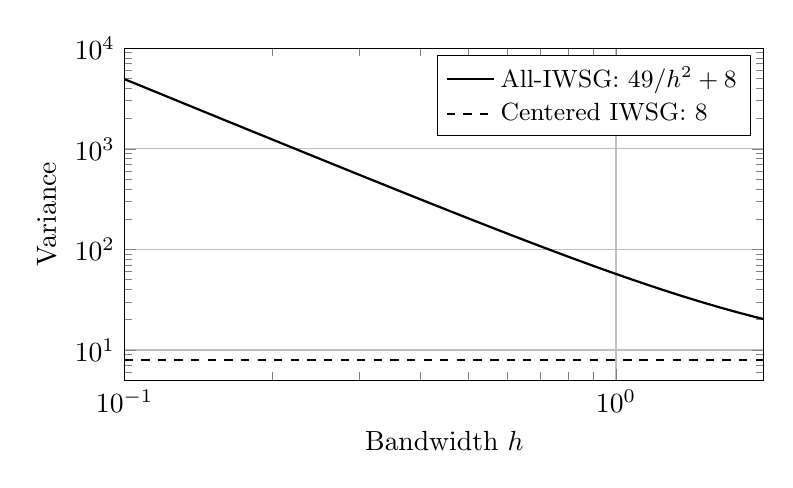
\begin{tikzpicture}
\begin{loglogaxis}[
 width=.80\textwidth,height=5.8cm,
 xlabel={Bandwidth $h$},ylabel={Variance},
 xmin=.1,xmax=2,ymin=5,ymax=10000,
 grid=major,legend style={at={(.98,.98)},anchor=north east,font=\small},
 legend cell align=left]
 \addplot[black,thick,domain=.1:2,samples=80]{49/(x*x)+8};
 \addlegendentry{All-IWSG: $49/h^2+8$}
 \addplot[black,dashed,thick,domain=.1:2]{8};
 \addlegendentry{Centered IWSG: $8$}
\end{loglogaxis}
\end{tikzpicture}
\caption{A narrow component can make an unbiased importance-weight derivative
noisy. For $a=2$, $\mu=3$, and $b=1$, the uncentered variance grows as
$49/h^2+8$, while the centered variance stays at 8. The pathwise derivative
has zero variance and therefore does not appear on the logarithmic axis.
These curves are the exact calculation in
\eqref{eq:gaussian-gradient-variance}, not filtering benchmark results.}
\label{fig:gradient-variance}
\end{figure}

This example isolates one smooth component. Younis's argument concerns an
additional difficulty: implicit mixture reparameterizations may move samples
between widely separated modes and have large variance. The example does
not refute that finding. It motivates treating continuous motion within a
component differently from a change in component probability.

\begin{samepage}
Let $m_\theta(z)=\sum_iw_i(\theta)k_{i,\theta}(z)$, sample
$I\sim\operatorname{Cat}(w)$, and represent a component sample by
$Z=T_{I,\theta}(\varepsilon)$ with parameter-independent base noise.
Assume positive component weights and sufficient regularity and integrability
to differentiate each component expectation. Differentiating their sum gives
\begin{align}
 J(\theta)&=\sum_iw_i\,
             \mathbb E_\varepsilon[\phi_\theta(T_{i,\theta}(\varepsilon))],
 \notag\\
 \nabla_\theta J
 &=\sum_i(\nabla_\theta w_i)\,
             \mathbb E_\varepsilon[\phi_\theta(T_{i,\theta}(\varepsilon))]
   +\sum_iw_i\,
             \mathbb E_\varepsilon\!\left[
                 \frac{d}{d\theta}\phi_\theta(T_{i,\theta}(\varepsilon))
             \right].
 \label{eq:hybrid-component-derivation}
\end{align}
\end{samepage}
For a baseline $c$ independent of the current component and noise, a resulting
estimator is
\begin{equation}
 G_{\rm hybrid}
 =\frac{d}{d\theta}\phi_\theta(T_{I,\theta}(\varepsilon))
  +(\phi_\theta(Z)-c)\nabla_\theta\log w_I.
 \label{eq:hybrid-estimator}
\end{equation}
The first term holds $I$ fixed and includes both the explicit derivative of
$\phi$ and movement of $T_{I,\theta}$. The second accounts for changing
component probabilities. Its baseline has zero expectation because
$\sum_iw_i\nabla\log w_i=\nabla\sum_iw_i=0$. A component-dependent baseline
does not have this cancellation unless its compensating term is retained.
The baseline may depend on $\theta$ or past information, but it is held fixed
within this gradient-estimation operation.

The categorical term can be averaged over its conditional component
responsibilities, or components can be enumerated and sampled with a
stratified allocation. Such changes have different costs and covariances with
the pathwise term. Reducing the variance of one term does not automatically
rank the complete estimator. A baseline fitted from the same sample also
requires a justified leave-one-out or independent-fit construction; otherwise
the claimed zero-mean property can fail.

The official Younis code contains an
\texttt{ImportanceImplicitHybrid} branch that separates derivatives of
component locations/bandwidths from derivatives of weights
\citep{youniscode2023}. Its continuous part uses implicit mixture
reparameterization. Equation~\eqref{eq:hybrid-estimator} instead uses a
componentwise pathwise derivative and is a distinct proposal. Neither the
presence of that branch nor the single-Gaussian calculation establishes
benefit for the full BayesFilter recursion.

Finally, the identity being estimated must remain explicit. A hybrid may
estimate the same mixture expectation derivative as IWSG while differing
sample by sample. Substituting it into a fixed-anchor finite program and
claiming the same derivative would require a new argument. The finite
program, the expected stochastic objective, and the underlying model score
cannot share a name merely because their estimators agree in a small example.

\subsection{What a control variate can accomplish}

For a baseline score estimate $G$ and a control $C$ with known mean $c$, define
\begin{equation}
 G_{\rm cv}=G-\beta(C-c),\qquad
 \mathbb E G_{\rm cv}=\mathbb E G.
 \label{eq:score-control-variate}
\end{equation}
The equality requires fixed $\beta$, or suitable independence from the
current estimating sample. A vector control may use a coefficient matrix.
A useful correlation can reduce variance and hence MSE, but the baseline
bias is retained. An independently estimated $c$ can be used when its
expectation is correct and its additional uncertainty is included. Merely
naming a KDM score as the control does not provide its mean.

The earlier residual decomposition is still an exact algebraic identity:
\begin{equation}
 L_0^N=A_h+\left(L_0^N-A_h\right),\qquad
 \dd L_0^N=\dd A_h+\dd\left(L_0^N-A_h\right).
 \label{eq:residual}
\end{equation}
Dropping the residual changes the target. Computing both terms exactly,
however, gives the original calculation back and supplies no automatic
variance or cost reduction. The useful additional ingredient would be a
cheap, accurately integrable approximation and a residual whose expectation
can be estimated with less error or work.

For example, let $\widetilde p_\theta(x,y)$ be a tractable approximation to
the joint density, with known integral $\widetilde Z(\theta)$. For a proposal
$q$ covering the support of the density difference,
\begin{align}
 Z(\theta)&=\widetilde Z(\theta)
 +\mathbb E_q\!\left[
       \frac{p_\theta(X,y)-\widetilde p_\theta(X,y)}{q(X)}\right],\\
 \nabla_\theta Z(\theta)&=\nabla_\theta\widetilde Z(\theta)
 +\mathbb E_q\!\left[
       \frac{\nabla_\theta p_\theta(X,y)
             -\nabla_\theta\widetilde p_\theta(X,y)}{q(X)}\right].
 \label{eq:joint-surrogate-residual}
\end{align}
The second equality assumes fixed $q$ and valid differentiation under the
integral. If the approximation is close, the residual may be easier to
integrate. The ratio of the resulting estimates still need not be an unbiased
score, and a signed residual estimate can make the likelihood estimate
negative. It is therefore not automatically eligible for pseudo-marginal
inference. The residual formulation deserves a separate comparison if a
tractable approximation can be constructed cheaply; it is not what the
previous integrated KDM experiments implemented.


\section{Other options and their place in the investigation}
\label{sec:alternatives}

Analytic marginalization should come before additional approximation when
the model permits it. Section~\ref{sec:model-mixtures} gives the one-step
Gaussian example. A conditionally linear-Gaussian state block can similarly
be integrated rather than sampled, provided its conditional model is retained
exactly. A Gaussian approximation to a nonlinear block is a different choice
and needs its own error assessment. Neither a good fit to state observations
nor an appealing proposal density establishes that the downstream score is
accurate.

More particles, paired random designs, and randomized quasi-Monte Carlo are
important equal-compute alternatives. They can improve integration without
changing the scientific target, but they cannot restore a missing derivative
or correct a filtering approximation with persistent bias. The comparison
must distinguish a better estimator from simply spending more work on it.
Sparse mixtures, low-rank density approximations, and approximate backward
sums likewise require separate bias and cost measurements; they are not
algebraically equivalent to the full mixture merely because they produce
finite values.

Bandwidth or particle-count extrapolation is another possible bias-reduction
strategy, but it requires a justified expansion. A presumed $h^2$ smoothing
bias or $1/N$ score bias cannot be used across every nonsmooth, constrained,
or resampling model without evidence. Randomized telescoping is more general.
For coupled levels $S_l$ and an independent random truncation $L$,
\begin{equation}
 \widehat S_{\rm tel}
 =S_0+\sum_{l=1}^{L}\frac{S_l-S_{l-1}}{\Pr(L\ge l)},
 \qquad
 \mathbb E\widehat S_{\rm tel}=\lim_{l\to\infty}\mathbb E S_l,
 \label{eq:randomized-telescope}
\end{equation}
when absolute integrability permits exchanging sum and expectation. The
expectation equality follows because each retained increment has inclusion
probability $\Pr(L\ge l)$. The limit must first be shown to equal the model
score. Finite expected work and finite variance impose additional conditions
on the coupling and truncation tail; the displayed equality supplies neither.
This makes literal unbiasedness a distinct research problem rather than a
promised property of the next mixture prototype.

The original proposal-force use remains valid in a different role. A
deterministic position-only field may generate a reversible,
volume-preserving kick--drift--kick proposal, with acceptance computed from
the declared endpoint Hamiltonian. Each kick and drift is a shear with unit
Jacobian determinant. Reversing the step size reverses the sequence, and a
momentum flip turns the symmetric sequence into an involution. The ordinary
Metropolis ratio therefore corrects this proposal for the endpoint density;
the force need not be its exact gradient. If the endpoint uses a fixed
finite-particle likelihood, it preserves that approximate target, not the
exact state-space posterior. Exact pseudo-marginal inference instead needs a
valid nonnegative unbiased likelihood estimate and the auxiliary randomness
in the extended target. A new random score at each leapfrog step is not
automatically a reversible proposal.

The BayesFilter HMC interface already distinguishes an exact score from a
frozen proposal field. A future raw-coordinate field must use the typed
endpoint-corrected binding with \texttt{tune\_hmc\_kernel}; the
fixed-transport tuner is for a genuine frozen coordinate transport with its
Jacobian-corrected target. This document does not change an HMC consumer or
claim posterior readiness. The interface and capability registry were read
to keep the proposed downstream use consistent with the actual repository.

The practical order is therefore to check model identity and complete
initialization, establish a corrected mixture/Fisher reference, compare
selective gradient estimators where needed, and then investigate scalable
ancestor approximations or learned proposals. Control variates, analytic
integration, and increased integration effort should be evaluated alongside
that sequence. Further structural DSGE implementation remains deferred while
the existing repository models are checked; the support derivations below
are retained because they explain which model extensions will be valid.


\section{Structural support and deferred extensions}
\label{sec:support}

The relevant support belongs to the distribution being approximated.
Deterministic directions in a transition conditional on one ancestor do not,
by themselves, imply that the predictive or filtering marginal lies on a
lower-dimensional surface.  For example, consider the state
$x_t=(m_t,m_{t-1})$ of an AR(2) process with independent standard normal
innovations $\varepsilon_t$, so that
\begin{equation}
 x_t=A x_{t-1}+G\varepsilon_t,\qquad
 A=\begin{bmatrix}\phi_1&\phi_2\\1&0\end{bmatrix},\quad
 G=\begin{bmatrix}\sigma\\0\end{bmatrix},\quad
 [G,AG]=\begin{bmatrix}\sigma&\phi_1\sigma\\0&\sigma\end{bmatrix}.
 \label{eq:ar2-support-distinction}
\end{equation}
Conditional on $x_{t-1}$, the transition has rank-one covariance and fixes
$x_{t,2}=x_{t-1,1}$.  Starting from a known initial state, the covariance
after two independent shocks is $GG^\mathsf{T}+AGG^\mathsf{T}A^\mathsf{T}$.
It is positive definite when $\sigma\ne0$, because the displayed matrix has
determinant $\sigma^2$.  Multiplication by a strictly positive Gaussian
observation likelihood does not reduce that marginal support.  Earlier
uncertainty can therefore fill directions that receive no new shock at the
current time.

For finitely many fixed ancestors, however, the conditional mixture in this
example lies on parallel lines with different offsets $x_{t,2}=x_{t-1,1}^i$.
These components do not have one common affine support.  A shared tangent
basis alone cannot justify evaluating all their densities at every ambient
sample as though their offsets agreed.  Nor does a reset of the filtering
marginal necessarily retain a particular old ancestor: a constraint on the
two-slice pair $(x_{t-1},x_t)$ must not be imposed without that conditioning.
Consequently, support must be checked separately for the transition factor,
the KDM insertion distribution, and the reset output.

When the distribution to be approximated does have a common affine support,
a constrained construction injects noise through its stochastic coordinates:
\begin{equation}
 u=G_\theta L_\beta\varepsilon,\qquad
 B_\theta=G_\theta H_\beta G_\theta^\mathsf{T},\qquad
 \varepsilon\sim N(0,I).
 \label{eq:innovation-kernel}
\end{equation}
For a linear support constraint $D x=c$, the kernel must satisfy
$D G_\theta=0$.  For a nonlinear manifold, a chart or retraction
$x=\rho_\theta(v,\varepsilon)$ is required, together with the appropriate
coordinate-space density and Jacobian.  When $B_\theta$ is rank deficient,
there is no ordinary full-dimensional Lebesgue density.  The implementation
must evaluate the mixture in innovation or chart coordinates rather than
pretending that $B_\theta$ is a full SPD ambient covariance.

This constrained kernel is an extension motivated by the DSGE target, not a
claim from the Younis papers.  Its first tests are rank, constraint residual,
and finite-difference tests for the $G_\theta$ and $H_\beta$ tangents.  A
positive bandwidth that leaves the support is a hard failure even if its
numerical score looks smoother.

The Phase~2 diagnostic implements the fixed-chart special case: a shared
orthonormal basis $U\in\R^{d\times r}$ is frozen, the Gaussian mixture is
evaluated in $U^\mathsf{T}x$ coordinates, and the orthogonal residual is checked
for both values and tangents.  This gives a rank-aware density with respect to
the chart measure for a fixed linear support.  It does not yet differentiate a
parameter-dependent $G_\theta$, chart, or retraction.  Moreover, a moving
support requires more than a density Jacobian.  A fixed ambient sample need
not remain on the support at neighboring parameter values, so the
fixed-ambient IWSG ratio used in the full-rank reference may cease to exist.

An exact example makes the missing term explicit.  Let $U\sim N(0,1)$,
$X_\theta=(U,\theta U)$, and $Y=X_\theta+V$, where $V\sim N(0,I_2)$ is
independent.  The state lies on a line that rotates with $\theta$, while the
observation has covariance
\begin{equation}
 C_\theta=\begin{bmatrix}2&\theta\\\theta&1+\theta^2\end{bmatrix},
 \qquad
 C'_\theta=\begin{bmatrix}0&1\\1&2\theta\end{bmatrix}.
 \label{eq:moving-support-covariance}
\end{equation}
The Gaussian score is
$\tfrac12\{y^\mathsf{T}C_\theta^{-1}C'_\theta C_\theta^{-1}y
-\operatorname{tr}(C_\theta^{-1}C'_\theta)\}$, which equals $1/2$ at
$\theta=0$ and $y=(1,1)$.  A sample $(u,0)$ anchored at zero lies outside
the perturbed line for every $u\ne0$ and $\theta\ne0$.  The two state laws
are mutually singular, so the perturbed law has no importance density with
respect to the anchor law.  The chart's arc-length factor is
$J_\theta=\sqrt{1+\theta^2}$; its logarithmic derivative is zero at the
anchor and cannot account for the nonzero observation score.

Keeping the innovation $u$ fixed instead gives a differentiable integral,
where $\phi$ is the standard normal density:
\begin{align}
 p_\theta(y)
   &=\int \phi(u)\,\mathcal N(y;(u,\theta u),I_2)\,\dd u,\\
 \frac{\partial p_\theta(y)}{\partial\theta}
   &=\int \phi(u)\,\mathcal N(y;(u,\theta u),I_2)
                 u(y_2-\theta u)\,\dd u.
 \label{eq:moving-support-score}
\end{align}
At zero, $E[U\mid Y=y]=y_1/2$, recovering the score $y_1y_2/2$.
The extra term comes from movement of the state inside the observation
factor, even though the innovation density is unchanged.

For a regular chart $x=\rho_\theta(v)$ on a fixed coordinate domain, let
$m_\theta(v)$ be the coordinate mixture density and $F_\theta(x)$ the
downstream likelihood integrand.  The corresponding differentiation rule is
\begin{align}
 I(\theta)&=\int F_\theta(\rho_\theta(v))m_\theta(v)\,\dd v,\\
 \partial_\theta I
 &=\int\!\left[
   (\partial_\theta F_\theta)(x)
   +\nabla_xF_\theta(x)^\mathsf{T}\partial_\theta\rho_\theta(v)
   +F_\theta(x)\partial_\theta\log m_\theta(v)
   \right]m_\theta(v)\,\dd v.
 \label{eq:chart-total-expectation}
\end{align}
This requires the usual integrability conditions for differentiating under
the integral.  An anchored proposal in $v$ can provide the raw mixture ratio,
but it cannot remove the chart-motion term.  If a surface-density convention
is used, its volume factor must be included consistently in the density and
measure.  Component-dependent supports require an explicitly defined common
measure or a mixed discrete and continuous formulation.

The affine specialization gives an explicit finite calculation in which all
these terms can be checked.  Suppose every component uses the same injective
chart $x=a_\theta+G_\theta v$, where $G_\theta\in\R^{d\times r}$ has full
column rank.  Let $v_j$ be fixed coordinate samples and let $q_0(v_j)>0$
be their frozen proposal density.  With coordinate means $c_i$, SPD
bandwidths $B_i$, and normalized positive weights $\alpha_i$, define
\begin{align}
 m_\theta(v)&=\sum_i\alpha_i\mathcal N(v;c_i,B_i),\qquad
 x_j=a_\theta+G_\theta v_j,\qquad
 \dd x_j=\dd a_\theta+(\dd G_\theta)v_j,
 \label{eq:affine-chart-state}\\
 b_j&=\frac{m_\theta(v_j)}{Nq_0(v_j)},\qquad
 \dd\log b_j=\dd\log m_\theta(v_j).
 \label{eq:affine-chart-iwsg}
\end{align}
Here $\dd$ denotes any one parameter-direction differential; multiple
directions obey the same equations.  All mixture components contribute.
Writing $z_{ji}=B_i^{-1}(v_j-c_i)$, the complete component and mixture
differentials are
\begin{align}
 \eta_{ji}&=\frac{\dd\alpha_i}{\alpha_i}
       +z_{ji}^{\mathsf T}\dd c_i
       +\frac12\left[z_{ji}^{\mathsf T}(\dd B_i)z_{ji}
                     -\operatorname{tr}(B_i^{-1}\dd B_i)\right],\\
 \gamma_{ji}&=\frac{\alpha_i\mathcal N(v_j;c_i,B_i)}{m_\theta(v_j)},\qquad
 \dd\log m_\theta(v_j)=\sum_i\gamma_{ji}\eta_{ji},\\
 \dd\gamma_{ji}&=\gamma_{ji}
                  \left(\eta_{ji}-\dd\log m_\theta(v_j)\right).
 \label{eq:affine-chart-mixture-differential}
\end{align}
No coordinate-sample differential appears because the $v_j$ are fixed.
The ambient state differential in \eqref{eq:affine-chart-state} generally
remains nonzero.

The surface-volume factor clarifies why it must not be added again to the
importance ratio.  Set $M=G_\theta^\mathsf{T}G_\theta$ and
$J_\theta=\sqrt{\det M}$.  Then
\begin{equation}
 \dd\log J_\theta=\tfrac12\operatorname{tr}(M^{-1}\dd M),\qquad
 \dd M=(\dd G_\theta)^\mathsf{T}G_\theta
                 +G_\theta^\mathsf{T}\dd G_\theta.
 \label{eq:affine-chart-volume}
\end{equation}
At the moving point $x_j$, the surface densities of the target and the
proposal pushed through the \emph{current} chart are respectively
$m_\theta(v_j)/J_\theta$ and $q_0(v_j)/J_\theta$.  Their ratio is
$m_\theta(v_j)/q_0(v_j)$: the common volume cancels.  The log target surface
density has differential $\dd\log m_\theta(v_j)-\dd\log J_\theta$, while
the log proposal surface density has differential $-\dd\log J_\theta$.
This construction uses a moving ambient proposal generated by fixed
coordinates; it does not assert that the perturbed law has a density relative
to the frozen ambient anchor law in the rotating-line counterexample.

The same chart can carry covariance marks when those marks are defined in
its coordinates.  For SPD coordinate marks $P_i^v$, define
\begin{align}
 \widetilde P_j^v&=\sum_i\gamma_{ji}P_i^v,\qquad
 \dd\widetilde P_j^v=\sum_i\bigl[(\dd\gamma_{ji})P_i^v
                                  +\gamma_{ji}\dd P_i^v\bigr],\\
 \widetilde P_j^x&=G_\theta\widetilde P_j^vG_\theta^\mathsf{T},\\
 \dd\widetilde P_j^x&=(\dd G_\theta)\widetilde P_j^vG_\theta^\mathsf{T}
       +G_\theta(\dd\widetilde P_j^v)G_\theta^\mathsf{T}
       +G_\theta\widetilde P_j^v(\dd G_\theta)^\mathsf{T}.
 \label{eq:affine-chart-marks}
\end{align}
The ambient mark is allowed to be singular.  These equations specify the
transport of marks defined in this common chart; they do not infer a full
DSGE UKF covariance lifecycle from a singular process covariance.

To expose the state-motion term at a consumer, take an observation
$y\mid x\sim\mathcal N(H_\theta x+o_\theta,R_\theta)$, with $y$ fixed and
$R_\theta$ SPD.  The finite log normalizer and its total differential are
\begin{align}
 \widehat L(\theta)&=\log\sum_j b_j g_\theta(y\mid x_j),\qquad
 \pi_j=\frac{b_jg_\theta(y\mid x_j)}{\sum_\ell b_\ell g_\theta(y\mid x_\ell)},\\
 \dd\widehat L&=\sum_j\pi_j
       \bigl[\dd\log m_\theta(v_j)+\dd\log g_\theta(y\mid x_j)\bigr].
 \label{eq:affine-chart-normalizer}
\end{align}
There is no subtraction of $\dd\log\sum_j b_j$; that would differentiate
a self-normalized finite value.  With
$e_j=y-H_\theta x_j-o_\theta$ and $s_j=R_\theta^{-1}e_j$, the observation
term is explicitly
\begin{equation}
 \dd\log g_\theta(y\mid x_j)
 =s_j^\mathsf{T}\bigl[(\dd H_\theta)x_j
                      +H_\theta\dd x_j+\dd o_\theta\bigr]
 +\tfrac12\left[s_j^\mathsf{T}(\dd R_\theta)s_j
               -\operatorname{tr}(R_\theta^{-1}\dd R_\theta)\right].
 \label{eq:affine-chart-observation}
\end{equation}
The term $H_\theta\dd x_j$ is exactly what a zero outgoing state tangent
would omit.  Differentiating this finite sum needs no exchange of derivative
and integral.  Relating it to a limiting likelihood still needs an importance
sampling argument and appropriate integrability conditions.  Its derivative
is neither the unchanged atom-program derivative nor, at finite $N$, the
exact model score.

Support preservation by the reset is a separate question.  On the parabola
$x=(u,u^2)$, a convex barycentre with weights $\lambda_i$ obeys
\begin{equation}
 \bar x_2-\bar x_1^2
   =\sum_i\lambda_i u_i^2-\left(\sum_i\lambda_i u_i\right)^2
   =\operatorname{Var}_\lambda(u).
 \label{eq:curved-support-barycentre}
\end{equation}
Thus even exact barycentric averaging leaves this curve whenever the weighted
variance is positive.  Contract--E adds residual injection and affine moment
restoration, so barycentric failure alone does not prove its final residual;
the actual reset must be evaluated.  On a common affine subspace, ambient
ridge and residual injection can likewise introduce normal-direction
variation.  Projecting the result or performing the reset in chart
coordinates changes the specified finite reset and requires its own
derivation; it cannot silently count as the existing Contract--E program.

The existing subspace kernel rejects points outside the rotating line,
and the independent observation-score check
recovers $1/2$ and its finite difference.  The affine equations above now have
a diagnostic implementation with a Gaussian observation consumer.  Its
two-direction tests perturb each mixture, chart, mark and observation input
separately and jointly.  The largest absolute difference from an independent
central-difference calculation is $6.11\times10^{-11}$ on these fixtures.
An executable wiring check follows that consumer to the existing complete
mixture evaluator.  Deliberately zeroing its outgoing state tangent changes
the computed normalizer derivative while leaving the value unchanged.

The reset probes are untuned CPU/float64 references, not measurements of
production filtering accuracy.  They use eight particles, Sinkhorn
$\epsilon=0.2$, 20 iterations plus five balance iterations, and ridge
$10^{-5}$, followed by the actual diagonal and pairwise correction with both
caps enabled.  On the line $x_2=0$, the maximum absolute constraint residual
is $0.00374$ after Contract--E and $6.52\times10^{-7}$ after correction.  On
$x_2=x_1^2$, the corresponding residuals are $0.918$ and $1.187$.  Both
correction calls return numerical validity.  That flag therefore does not
certify either of these support constraints.  These counterexamples concern
prescribed common supports; they do not impose an old ancestor's conditional
support on every filtering marginal.

The shared finite
LEDH executor still factors a full-rank process covariance and uses full-rank
Gaussian PF--PF factors.  A target-specific innovation-coordinate flow,
reset, density recurrence, and their analytical differentials must be
specified together before an end-to-end DSGE implementation can be claimed.
Its initial state and covariance tangents are also set to zero: a
parameter-dependent initial law requires explicit derivatives at that entry
point, whereas the completed reference campaigns held those inputs fixed.

\section{Implementation state and remaining gaps}
\label{sec:implementation}

The research snapshot and the main checkout must be distinguished. The
reported numerical results belong to research commit \texttt{804616e3}; the
main checkout inspected for this revision is \texttt{5cc59cfa}. The analytical
function and legacy batch wrapper are the two functions named in
Section~\ref{sec:atom}, with the source-route initialization in
\texttt{bayesfilter/highdim/ledh\_pfpf\_genut\_initial\_rqmc\_tf.py}.  The
existing prior-weight sidecar captures a corrected pre-observation cloud, but
it does not implement the Younis IWSG mixture gradient through the integrated
\LEDH{}--\OT{}--\GenUT{} reset.  It must not be relabelled as that method.

The registry call-chain repair is complete.  Phase~1 is now implemented as the
diagnostic module
\path{bayesfilter/highdim/ledh_younis_kdm_tf.py}.  Its route ID is
\begin{center}
\texttt{ledh\_younis\_kdm\_algebra\_}\texttt{diagnostic\_v1}
\end{center}
Its global and
conditional mixture kernels expose the all-pairs density and complete cloud,
weight, and covariance tangents.  The source-matched fixed-proposal IWSG
kernel has no sample-location tangent and keeps the proposal density at its
supplied anchor.  The conditional kernel is labelled as a proposal-density
evaluator, not a model-score estimator.  The separate anchored
\texttt{MODEL-IS} PF--PF kernel contains every value term in
\eqref{eq:kdm-proposal-density}--\eqref{eq:kdm-proposal-weight} and requires
an explicit per-particle certificate that the forward map is invertible; a
finite log determinant alone is not accepted as that certificate.  Its
tangent excludes proposal and selection derivatives because their sampling
law is frozen at the anchor.  The module is diagnostic-only and is not in the
canonical registry or call chain.

\begin{samepage}
The bounded Phase~1 test suite passes its complete-tangent, rank, anchor,
proposal, and XLA-smoke checks.  Phase~2A adds

\begin{itemize}[leftmargin=2em]
  \item the controlled one-step linear-Gaussian normalizer\\
        \texttt{make\_linear\_gaussian\_kdm\_}\\
        \texttt{normalizer\_kernel}, whose
        positive branch is \texttt{KDM-FINITE} and whose explicit zero branch
        is \texttt{ATOM-FINITE}; and
  \item an opt-in \texttt{return\_trace=True} surface on the analytical
        endpoint, used to build the sidecar from the actual post-flow cloud
        and weights under the Contract--E/dual-cap settings.
\end{itemize}
\end{samepage}

The Phase~2A finite-difference and endpoint tests pass, and the Phase~2B
fixed-chart support tests pass.  Phase~3 now provides
\texttt{canonical\_linear\_gaussian\_kdm\_auxiliary}.  It reads the actual
analytical trace, reconstructs the zero-bandwidth value and score from
\eqref{eq:prior-observation-factorization}, and reports a separately labelled
positive-bandwidth functional without feeding it into the reset.  In
particular, it uses $\bar w_t$, not $w_t^+$; using $w_t^+$ would apply the
current observation twice.

Phase~4A is now implemented in
\path{bayesfilter/highdim/ledh_younis_kdm_integrated_tf.py}.  The route
\texttt{ledh\_younis\_kdm\_integrated\_observation\_weighting\_v1} calls the
same internal finite-program executor as the registered canonical wrapper and
substitutes only the observation factor.  The code implements
\eqref{eq:linear-convolution-tangent}, feeds the resulting weights and
tangents through Contract--E and both correction caps, and returns the actual
multi-step trace.  Its fixed-shape factory defaults to XLA compilation.

The implementation audit also repaired three pre-existing total-derivative
gaps in the shared analytical executor: generic Gaussian transition and
observation fallbacks now include direct covariance-density tangents; a model
may supply the total tangent of its observation Jacobian; and every resulting
$\dd H$ term enters the LEDH flow.  The flow log determinant now uses an
XLA-compatible QR/triangular-solve identity rather than an unsupported matrix
determinant/inverse pair.  Rebuilt-model finite differences test these terms.

Phase~4A is a correct total derivative of its declared
\texttt{KDM-FINITE} scalar; it is wrong if described as the derivative of
\texttt{ATOM-FINITE}.  The current one-cell experiment gives no evidence that
it reduces model-score error, and the all-bandwidth inspection indicates that
its small variance reduction is offset by additional bias.  The complete
rows, manifest, and source hashes are recorded under
\path{docs/benchmarks/artifacts/ledh_younis_kdm_}\\
\path{phase4_20260908/campaign-attempt05-n32t5-all-rho-f32-current/}.

Phase~4B is no longer blocked by an unspecified mixture or ancestry rule:
Equations~\eqref{eq:phase4b-mixture}--\eqref{eq:phase4b-finite-target} define
the source-matched raw mixture ratio, the BayesFilter covariance marks,
the insertion point after Contract--E, and the two-pass anchor/replay rule.
The exact $N$-by-$N$ operation is implemented in
\path{bayesfilter/highdim/ledh_younis_kdm_resampling_tf.py}.  Its anchor and
replay endpoints call the shared canonical executor after Contract--E and both
correction caps, enforce one common full-rank Gaussian bandwidth at each time,
and expose both raw and self-normalized ratio diagnostics with complete
tangents.  The repaired route carries raw ratios divided by $N$, not
self-normalized ratios, into the next PF--PF normalizer.  The
responsibility-mean and fixed-label covariance-mark policies are separate,
explicit routes.  One-at-a-time and joint finite
differences, exact anchor replay, canonical no-hook parity, and isolated
two-step state/weight/covariance wiring tests pass.  Bounded float64 and
float32/no-TF32 GPU/XLA smokes of the earlier self-normalized route are
superseded for derivative certification.  On 9 September, four fresh smokes
of the repaired raw-IWSG program passed for both precisions and both covariance
mark policies at $D=2,N=8,T=2$.  These checks establish implementation
consistency for \texttt{RESKDM-IWSG-FINITE}.  The subsequent matrix campaign
supplies the separate negative model-score result reported above.  The
conditional \texttt{MODEL-IS} proposal
remains an extension and is not a substitute for this combined program.
The canonical trace now retains, rather than discards, higher-moment validity,
the off-diagonal target mask, pairwise pre/post-cap displacement, pairwise cap
scale, and coordinate-cap activity.  The new matrix Kalman recursion and
fixed-stream bootstrap comparator pass analytical-versus-finite-difference
tests.  A terminal audit reproduced both campaign summaries from the raw rows
and verified source hashes, split counts, validity flags, and complete
correction diagnostics.  Its receipts are retained under
\path{docs/benchmarks/artifacts/ledh_younis_kdm_phase4b_20260909/campaign01/}.
The campaign completed, but its planned power requirement was not met.  The
affine-chart diagnostic in
\path{bayesfilter/highdim/ledh_younis_kdm_affine_chart_reference_tf.py}
implements \eqref{eq:affine-chart-state}--\eqref{eq:affine-chart-observation},
including two-direction and heterogeneous-coordinate-mark tests.  All 35
focused CPU/float64 reference checks pass.  It is not wired into the
multi-step LEDH executor and has not been validated on GPU/XLA.  Further DSGE
implementation is deferred. The five-adapter checks below establish a useful
starting point for current model support. Before those models support any
new score-quality conclusion, their initial laws and precise observation and
transition targets must be resolved and the complete consuming filter tested
under fresh model-specific calibration.  An existing model
that the current executor cannot represent must remain explicitly untested;
it must not be replaced by a different full-rank model to fill a results table.

The first cross-model audit exposes why component fidelity is not enough.
The generalized-SV adapter evaluates the actual heteroskedastic likelihood,
but its flow also depends on the process covariance and on the observation
map.  Write its parameters as
$\theta=(a_s,a_h,\log\sigma_s,\log\sigma_h,\log\beta)$ and perturb them in
direction $v$.  The process covariance and flow observation map obey
\begin{align}
 Q&=\operatorname{diag}(\sigma_s^2,\sigma_h^2),
 &\dd Q&=\operatorname{diag}(2\sigma_s^2v_3,2\sigma_h^2v_4),\\
 H&=[\beta,0], &\dd H&=[\beta v_5,0],\\
 \dd(Hx)&=H\,\dd x+(\dd H)x.
 \label{eq:repository-gsv-flow-tangent}
\end{align}
Here parameter components are numbered from one.  The adapter previously
omitted $\dd Q$, $\dd H$, and the second term in the last line.  Correct
differentiation of the likelihood at a supplied state cannot restore those
missing derivatives of the state produced by the flow.  The KSC adapter had
the same problem with its flow observation offset: the differential of
$h+\mu_{\rm mix}+2\log\beta$ is $\dd h+2\dd\log\beta$, not just $\dd h$.
Finite differences that rebuild both adapters at the perturbed parameters
expose these omissions.  They are implementation errors relative to the
total-derivative claim, not evidence against KDM.  The KSC mixture must also
remain distinct from exact transformed SV: replacing log-chi-square noise by
seven Gaussian components changes the observation density, so an
observation-transform Jacobian does not imply equal scores.

After these repairs and a graph-construction repair for Austria SIR, the first
cross-model batch passes 39 checks.  All five existing adapters---diagonal
LGSSM, native generalized SV, KSC, predator--prey, and the current Austria SIR
recurrence---pass coordinate-by-coordinate and mixed-direction finite
differences through the two-step canonical and raw-IWSG replay endpoints.
The largest scaled discrepancy is $2.50\times10^{-8}$.  These are CPU/float64
reference tests with fixed initial clouds and covariances.  The executor still
initializes their tangents to zero, whereas a stationary SV initial law depends
on its persistence and innovation scale.  Its total model-score derivative
therefore needs additional initialization terms.  The continuous SIR
recurrence also omits the susceptible clipping in the repository simulator
and its latent-preclip representation.  Its derivative test does not establish
either model identity.  Both discrepancies must be resolved before those
models enter the score-accuracy comparisons; the remaining repository models
are still untested by this batch.

Fresh Phase~4A endpoint calibration after the covariance-carry repair passes
for float64 and for float32 without TF32.  Its float32 TF32 arm still fails the
declared graph/XLA and atom-identity tolerances, so TF32 remains unadmitted for
that diagnostic route.  Phase~4B has so far been checked only in float64 and
float32 without TF32.  The batch implementation has changed since the earlier limitation was
written. In the inspected main checkout,
\path{ledh_canonical_batch_fused_tf.py} now calls the single-cloud analytical
executor and forwards Contract--E, higher-moment, pairwise-cap, and
coordinate-cap settings. It uses nested \texttt{tf.map\_fn} calls over rows
and parameter directions. This is a row-mapped scalar implementation; despite
the filename and its description, it does not satisfy the repository's
requirement for a batch-native NeuTra training target. The older
\path{ledh_canonical_batch_tf.py} wrapper also maps rows and does not itself
forward a Contract--E reset selection, so its default invocation remains the
diagnostic reset-free slice.

The shared main-checkout score executor now reaches
\texttt{batched\_higher\_moment\_shape\_jvp} in
\path{ledh_unified_correction_tf.py} through a batch-axis adapter. This source
change means the old experiment hashes cannot certify the current shared
numerics. Source wiring was inspected for this revision; numerical parity of
that later dependency chain was not rerun. The integrated observation and
raw-IWSG source files match the research snapshot, but their shared dependency
has changed. Implementation reuse is therefore distinct from renewed
numerical certification.

The new marginal proposal, ancestor-averaged Fisher recursion, and selective
component gradient in Sections~\ref{sec:model-mixtures}--\ref{sec:hybrid}
are derived proposals. They are not integrated, tested runtime candidates in
either snapshot. The existing anchored \texttt{MODEL-IS} kernel is a
one-step diagnostic and supplies only part of that future implementation.
A useful model-score estimator could differ from the derivative of
\eqref{eq:atom-program}; its value would be established against the underlying
model score and through its own implementation checks. The present results
establish neither HMC readiness nor a change to the canonical default.

\subsection{Checks on the existing finite-program endpoints}

The existing TensorFlow diagnostics reconstruct the Younis mixture
algebra with analytical tangents.  The proposal-corrected LEDH arm is a
separate extension, not a source theorem.  The evaluator must expose cloud,
weight, and bandwidth derivatives and provide a small all-pairs reference.  Any integrated claim requires the consuming endpoint to call the evaluator
with compatible shapes, dtypes, and derivatives. The proposed model-score
routes may have their own endpoints; a standalone density helper does not
establish integration with any complete filter.

The finite-program checks have the following distinct purposes:
\begin{enumerate}[leftmargin=2em]
  \item For Phase~4A, at zero bandwidth, value and score match the canonical
        fixed-stream program within the declared numerical tolerance.
  \item The Phase~4A zero-bandwidth branch is an atom calculation; no Cholesky
        factor or inverse of a zero covariance is used to manufacture the
        limit.  Phase~4B makes no zero-bandwidth parity claim.
  \item At positive bandwidth, the result records
        $\overline L_h^N-L_0^N$ and is not labelled value-preserving.
  \item Finite differences of the declared $L_h^N$ agree with its complete
        analytical tangent when state, observation matrix, process and
        observation covariances, bandwidth, and model parameters are
        perturbed separately and jointly.
  \item Before any future degenerate DSGE extension is admitted, its fixture
        must have zero support violation and a correct rank-aware density
        calculation.  That extension is deferred while existing repository
        models are tested.
  \item Any route claiming linear cost needs a scaling check with its stated
        assumptions; an all-pairs $N^2$ operation is incompatible with that
        claim.  The all-pairs implementation remains diagnostic.
  \item On a linear-Gaussian model, score error is compared with the Kalman
        score over paired paths and independent fixed streams.  Bias and
        variance are reported separately.
  \item For a \texttt{MODEL-IS} arm, the proposal-density identity is checked
        separately from the post-reset finite value; the complete mixture
        denominator, support, and forward Jacobian must all be present.
  \item For Phase~4B, every anchor sample is replayed exactly, its forward
        importance ratio is one, every component contributes to the
        marginalized density, and the $N^2$ responsibility and covariance-mark
        tangents agree with finite differences.
  \item The sequential Phase~4B endpoint is tested at $T\ge2$ so that the
        post-reset KDM state, weight, and covariance marks demonstrably affect
        a later normalizer.  A one-step density helper is not integration
        evidence.
  \item The next PF--PF step consumes the raw IWSG log weights and their
        uncentered tangents from \eqref{eq:phase4b-incoming-weight}; executable
        ablations must detect either one being discarded or prematurely
        normalized.
  \item The score-quality fixture has at least two state dimensions.  Its
        executed trace must contain a nonzero off-diagonal pairwise target mask,
        a finite nonzero pairwise correction displacement, and both pairwise and
        coordinate-cap diagnostics.  Merely setting nonzero options in a scalar
        model does not execute the pairwise algorithm.
\end{enumerate}

\section{The next discriminating comparison}
\label{sec:next-study}

The primary question is whether model-corrected mixture proposals and
ancestor averaging reduce model-score error at equal compute. Proposal
quality, score construction, and mixture-gradient variance must be separated.
Otherwise a successful run could be attributed to the wrong mechanism, just
as a passing derivative check previously obscured a changed scalar.

The smallest useful sequence begins with three calculations. First, compare
\eqref{eq:model-marginal-weights} and
\eqref{eq:fully-adapted-mixture} with direct Gaussian integration on a fixed
incoming cloud. Second, compare the complete-data and backward-recursion
scores with exact enumeration on a small finite-state model, including a
parameter-dependent initial law. Third, compare IWSG, centered IWSG, and
\eqref{eq:hybrid-estimator} for the same declared mixture expectation.
These calculations test identities and failure mechanisms; their particle
counts need only be large enough to exercise the operation being tested.
They are not score-quality campaigns or reasons to select a production
particle count.

The subsequent accuracy study should use a linear-Gaussian model with an
independent Kalman score, a short Gaussian-mixture model whose modes can be
enumerated exactly, and a scalar nonlinear model with a numerically converged
quadrature score. Kalman checks the basic integration and complete derivatives.
The mixture model tests the separated modes that motivate Younis's method.
The nonlinear model tests how proposal approximation affects the result.
A one-step or unimodal success cannot establish the latter two properties.
Models with unresolved initialization or support identity must be repaired
before their score results are interpreted.

For each model, change one mechanism at a time: ordinary ancestor sampling
versus marginal mixture weights; a genealogical complete-data score versus
the full ancestor average; and, where an expectation derivative is actually
used, all-IWSG versus the selective estimator. Include the enhanced
combination only after the component comparisons. The exact full-mixture
reference remains necessary when evaluating a later sparse or sampled
approximation.

The cheap alternatives are constructed from the model before claim data are
examined. A bootstrap PF proposes from the physical transition and uses a
proper complete-data score estimator. A locally adapted PF uses the current
observation to guide each ancestor's proposal and keeps the exact importance
weight. In nearly linear regimes, EKF and UKF approximate-likelihood scores
test whether inexpensive Gaussian propagation already suffices; their
derivatives must include the full declared Gaussian approximation. A
scope-tuned canonical LEDH filter supplies the project comparator. The exact
Kalman, mixture-enumeration, or quadrature solution supplies the oracle.
Neither a weak fixed-ancestry derivative nor an untuned numerical default
should stand in for all conventional particle-score methods.

Evaluate these comparisons conditionally. Weak and strong observations probe
proposal concentration; overlapping and separated modes probe mixture
gradients; low and high persistence probe loss of ancestor diversity; short
and long horizons probe accumulation; near-zero and large score components
probe the error scale. These situations must be defined from the model and
research question before using validation data. Failure against a cheap
alternative in a salient situation rejects promotion under the repository's
sanity-check rule, even if the method wins an unconditional average. The
adversaries are falsification checks, not extra tuning targets.

For dataset $d$ and independent filter randomization $r$, denote the estimate
by $\widehat s_{d,r}$ and the oracle by $s_d$. Replication within each fixed
dataset estimates $b_d$ and $V_d$ from
\eqref{eq:conditional-score-error}; the distribution over datasets measures
generalization. Pair methods within datasets and respect this nesting in
confidence intervals. A path bootstrap with only one filter realization per
path cannot estimate each dataset's conditional bias. Freeze parameter
coordinate scales before comparison, because a relative error divided by a
nearly zero oracle score is unstable. Change $N$ and $T$ independently, and
report both equal-particle and equal-measured-compute comparisons.

Before a serious run, choose a practically meaningful reduction $\delta$ and
test a predeclared upper confidence bound for
\begin{equation}
 \Delta=\mathbb E\!\left[
    \|\widehat s_{\rm candidate}-s\|_D^2
    -(1-\delta)\|\widehat s_{\rm comparator}-s\|_D^2\right],
 \qquad \|v\|_D^2=v^\mathsf T Dv,
 \label{eq:next-study-criterion}
\end{equation}
where $D$ is the fixed coordinate scaling and the expectation follows the
specified sampling of datasets and filter randomizations. The upper bound must be below
zero, subject to validity and conditional-comparison vetoes. The old ten
percent criterion is not automatically a justified threshold for every new
model. Its practical meaning, replication requirement, multiplicity handling,
and total compute budget must be stated for the new study. A power pilot that
requires more replications than the budget permits leads to an inconclusive
study, not a forced ranking among viable candidates.

All material numerical choices need a provenance and failure explanation.
The physical transition covariance comes from the model; proposal bandwidth,
defensive-mixture fraction, covariance marks, chart, regularization, and
ancestor-sampling precision are numerical hypotheses. The earliest checks
should expose wrong support, missing proposal mass, large importance ratios,
or a gradient dominated by inverse bandwidth. Calibration and validation
must be disjoint for each bound model/horizon/particle/backend scope. The
initial law is part of that scope. Retaining an old setting for comparability
does not make it a tuned default, and a failed holdout cannot become the next
calibration set.

Numerical validity is assessed before score ranking. Nonfinite values,
incorrect density ratios, support violations, missing initial-law terms,
an invalid reference, or an omitted sampling-law derivative invalidate the
affected comparison. ESS, mode overlap, cap activity, tangent norms, bandwidth,
memory, and runtime explain its behavior; they do not replace the model-score
criterion. A valid candidate that loses is a candidate rejection. A later
prespecified repair may continue unless the target, evidence, or total budget
has become invalid.

BayesFilter implementation remains TensorFlow/TFP with analytical recursive
scores. Autodiff and finite differences are independent diagnostics. The
production direction remains GPU/XLA with the declared memory-growth and
transport-chunk policies; the earlier float64 and no-TF32 tests are reference
exceptions. New mixture evaluation must expose its pair count and memory
behavior. Batch wrappers must preserve the mathematical calculation and,
for NeuTra training, actually evaluate a batch rather than apply a scalar
target independently to each row. None of the proposed new calculations is
promoted by this document.

The most useful next evidence is therefore modest but decisive: correct
model-density weights and complete initialization, an independently checked
score recursion, and a powered comparison against simple alternatives. The
strongest alternative explanation for any improvement is better proposal
adaptation or more effective computation, rather than the gradient identity.
The component comparisons distinguish those explanations. Loss to a tuned
conventional score estimator at equal compute would overturn the practical
priority of the new combination without invalidating its algebra.


\appendix
\section{Source and experiment locations}

The original Section~3.6 manuscript is
\path{docs/papers/section_3_6_prior_weight_sidecar/section_3_6_prior_weight_sidecar.tex}
in the retained worktree
\path{.claude/worktrees/section-3-6-prior-weight-sidecar/}.
The present manuscript is
\path{docs/papers/ledh_younis_kdm_score/ledh_younis_kdm_score.tex}.
The protected source for this revision was recovered from commit
\path{804616e320d940a5ea288ba25cc43bd21d267abb} on
\path{kdm-total-score-continuation-20260909}. The main checkout was
\path{5cc59cfa26b8dec2b5a9e46497ef5639f2bfdb97}.

Phase~4A records are under
\path{docs/benchmarks/artifacts/ledh_younis_kdm_phase4_20260908/}; the
corrected all-bandwidth diagnostic is
\path{campaign-attempt05-n32t5-all-rho-f32-current/}.
Phase~4B records are under
\path{docs/benchmarks/artifacts/ledh_younis_kdm_phase4b_20260909/campaign01/}.
These paths describe the research snapshot and retained research worktree;
their absence from another checkout is not evidence that the experiment did
not run. The recovered numerical evidence and primary-source ledger are in
\path{docs/plans/artifacts/younis-score-recovery-20260911/}.
The accompanying scientific analysis is
\path{docs/plans/younis-model-score-analysis-2026-09-11.md}.

The derivations imported from the literature were checked at the following
locations: Younis and Sudderth (2023), Section~4, equations (14)--(15), and
the official resampling code; Younis and Sudderth (2024), Sections~2.3 and~4,
including the generative and learned smoother weights; Lai et al. (2022),
Algorithm~2, Theorem~2, equations (9)--(13), and the author's full-mixture
importance weights; Poyiadjis et al. (2011), Section~2.2, Algorithm~2,
equations (20) and (22); \citet[Section~4.2, equations (24)--(25)]{scibior2021dpf};
and Olsson and Westerborn, Section~3.1, Algorithm~2, and Section~3.2.4,
Theorem~10 with its mixing assumptions. Local paper copies are retained under
\path{.localresources/papers/}. These sources support the component
constructions; their combination with the proposed BayesFilter model-score
comparison remains to be evaluated.

The revision's protected baseline, source archive, equation-preservation
review, exact arithmetic examples, implementation wiring inspection, and
PDF build records are retained under
\path{docs/plans/artifacts/younis-manuscript-update-20260911/}.
This revision added analysis and exposition, and ran document and reference
checks. It launched no new particle-filter experiment.


\clearpage
\bibliographystyle{plainnat}
\bibliography{ledh_younis_kdm_score}

\end{document}
